\documentclass[draft]{beamer}

\usepackage{fontspec,xunicode,xltxtra}
\usepackage[english]{babel}
\usepackage{microtype}
\usepackage{default}	

\usepackage[]{hyperref}
\hypersetup{
	colorlinks=true}
\usetheme{simple}
\usepackage{graphicx}
\usepackage[utf8]{inputenc}
\usepackage[justification=centering]{caption}
\usepackage{subcaption}
\usepackage{listings}
\usepackage{pstricks}
\setmainfont{Fira Sans}
\setsansfont{Noto Sans}
\setmonofont{Fira Mono}
\captionsetup[subfigure]{labelformat=empty}
\captionsetup[figure]{labelformat=empty}
\setbeamertemplate{caption}{\raggedright\insertcaption\par}
\setbeamerfont{frametitle}{size=\LARGE}
\newfontfamily\DejaSans{DejaVu Sans}
\setbeamerfont{title}{family=\texttt,size=\huge}
\usepackage[scale=2]{ccicons}
\newfontfamily\unicodefun[Ligatures=TeX]{Symbola}
\newfontfamily\unicodefun{Droid Sans}
\title{Rethinking the DAW paradigm}
\subtitle{With i-score \& the LibAudioStream}
\date{}
\author{Jean-Michaël Celerier~\\ Myriam Desainte-Catherine~\\ Jean-Michel Couturier}
\institute{LaBRI, Blue Yeti}

\newsavebox{\codebox}% For storing listings
\begin{document}
    
\maketitle
\begin{frame}
	\tableofcontents
\end{frame}
\section{Introduction}

\begin{frame}
    \frametitle{DAWs}    
    \Large
    \begin{figure}
        \centering
        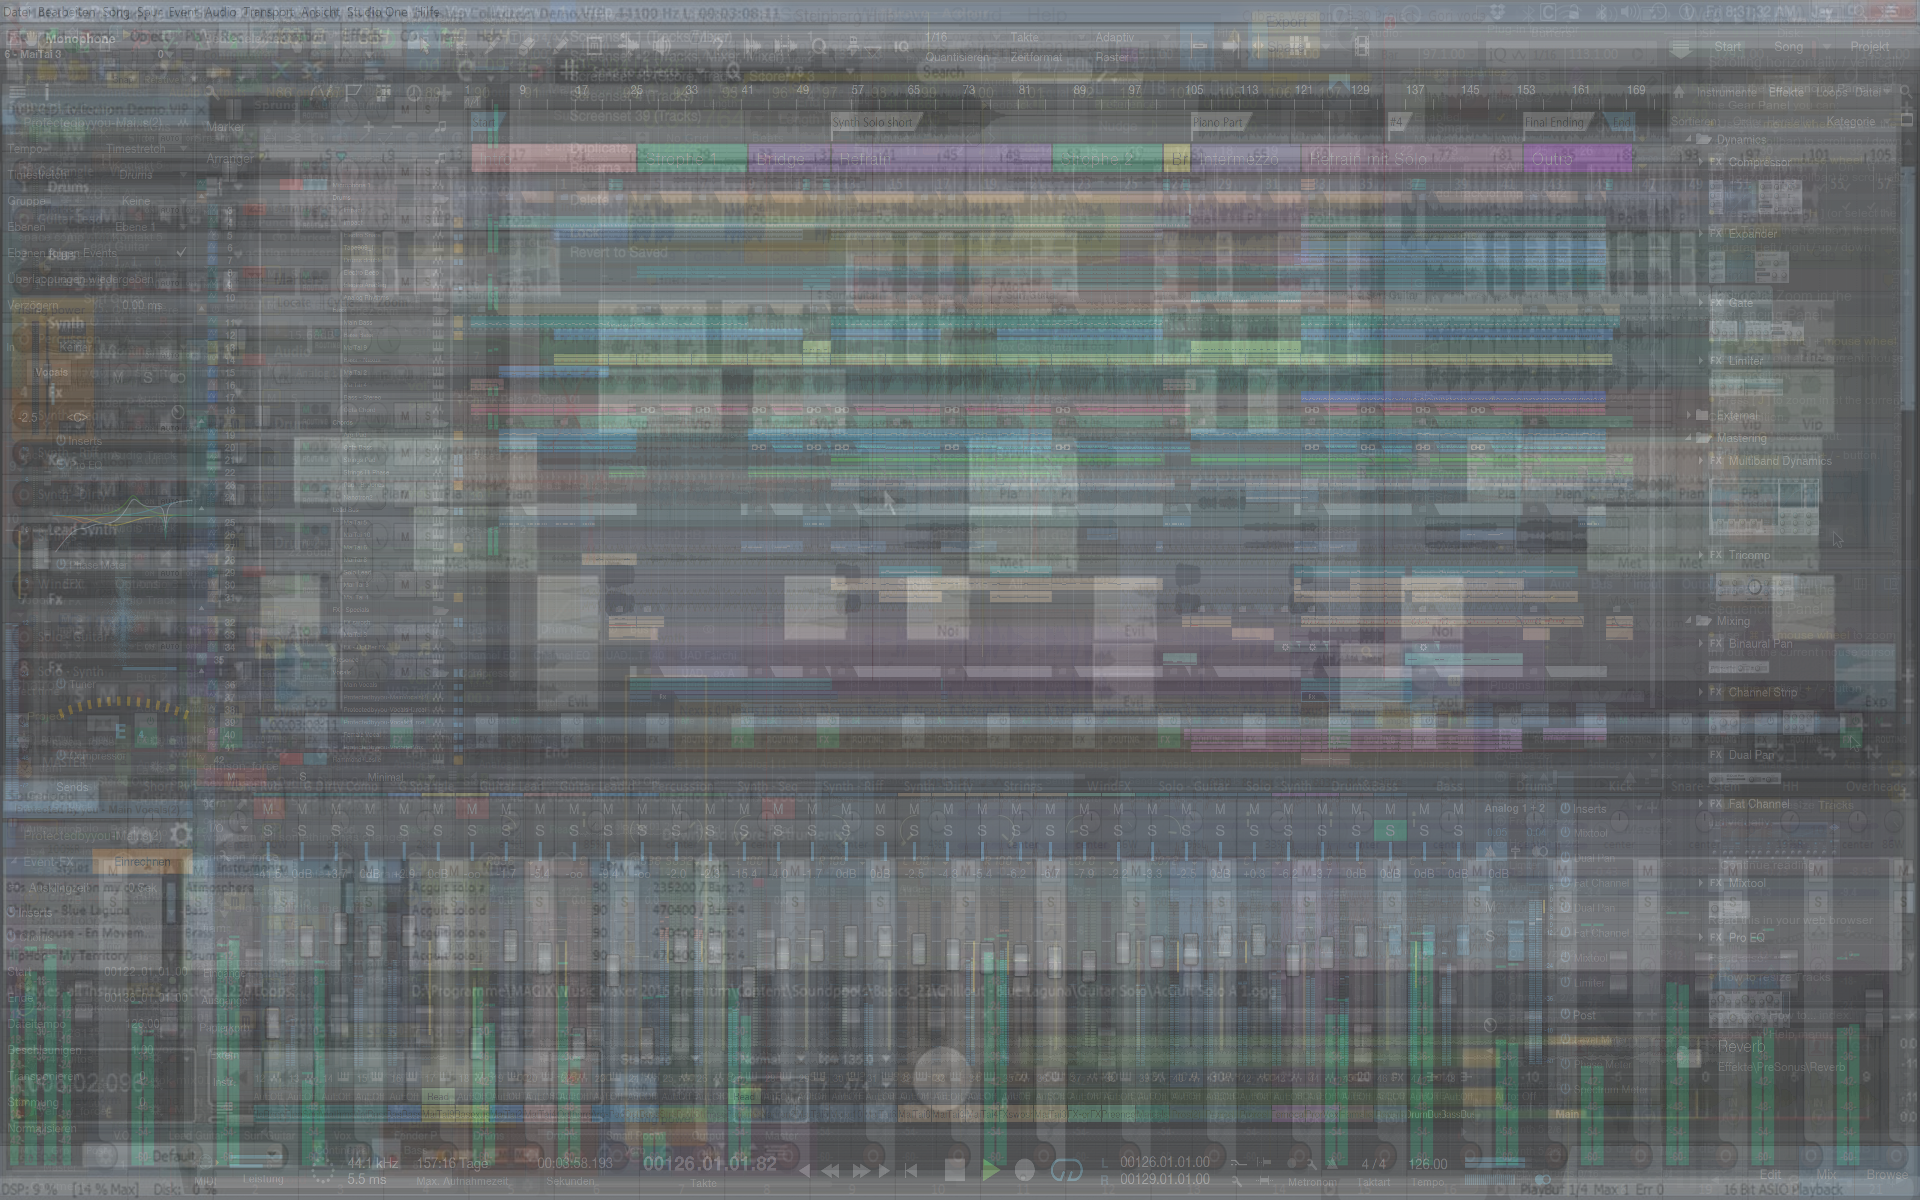
\includegraphics[width=0.9\textwidth]{images/daws/together-flattened.png}
        \caption{"Mixing"}
    \end{figure}
\end{frame}

\begin{frame}
    \frametitle{DAWs}    
    \Large
    \begin{figure}
        \centering
        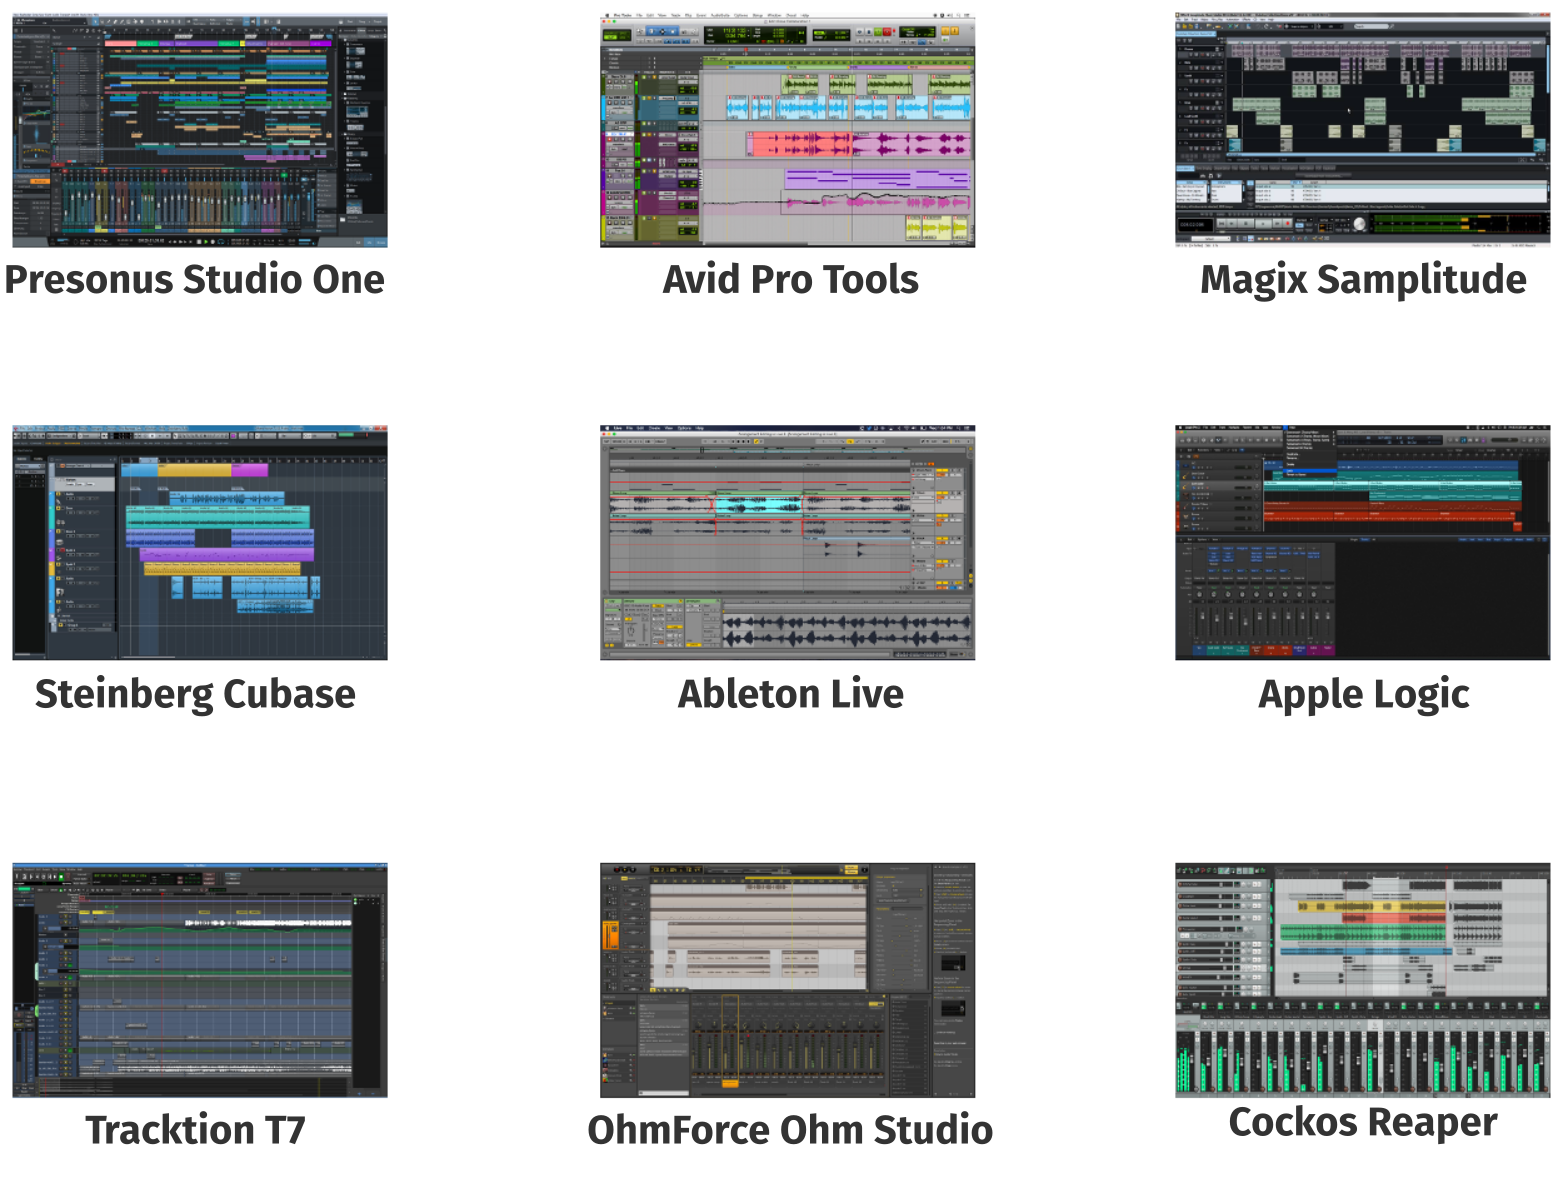
\includegraphics[width=0.7\textwidth]{images/daws/together-text.png}
        \caption{Pre-mix}
    \end{figure}
\end{frame}

\begin{frame}
	\frametitle{Music software UIs}    
	\Large
	\begin{itemize}
        \item<1-> Skeuomorphic (Most DAWs).
		\item<2-> Dataflows (\textbf{PureData}, \textbf{Max}, \textbf{OpenMusic}, \dots)
		\item<3-> Text (\textbf{Csound}, \textbf{ChucK}, \textbf{SuperCol}, \textbf{Nyquist}, \dots)
		\item<4-> Sometimes multiple possibilities~\\ (\textbf{Kyma}, \textbf{Antescofo}, \dots)
        \item<5-> Many others !
        \item<6-> Most are open for extensibility.
	\end{itemize}
\end{frame}

\begin{frame}
    Graphe échelle d'interactivité
\end{frame}
\begin{frame}
	\Huge
    \centering
    \textbf{What if...}
\end{frame}


\begin{frame} 
    \Large
    \begin{figure}
        \centering
        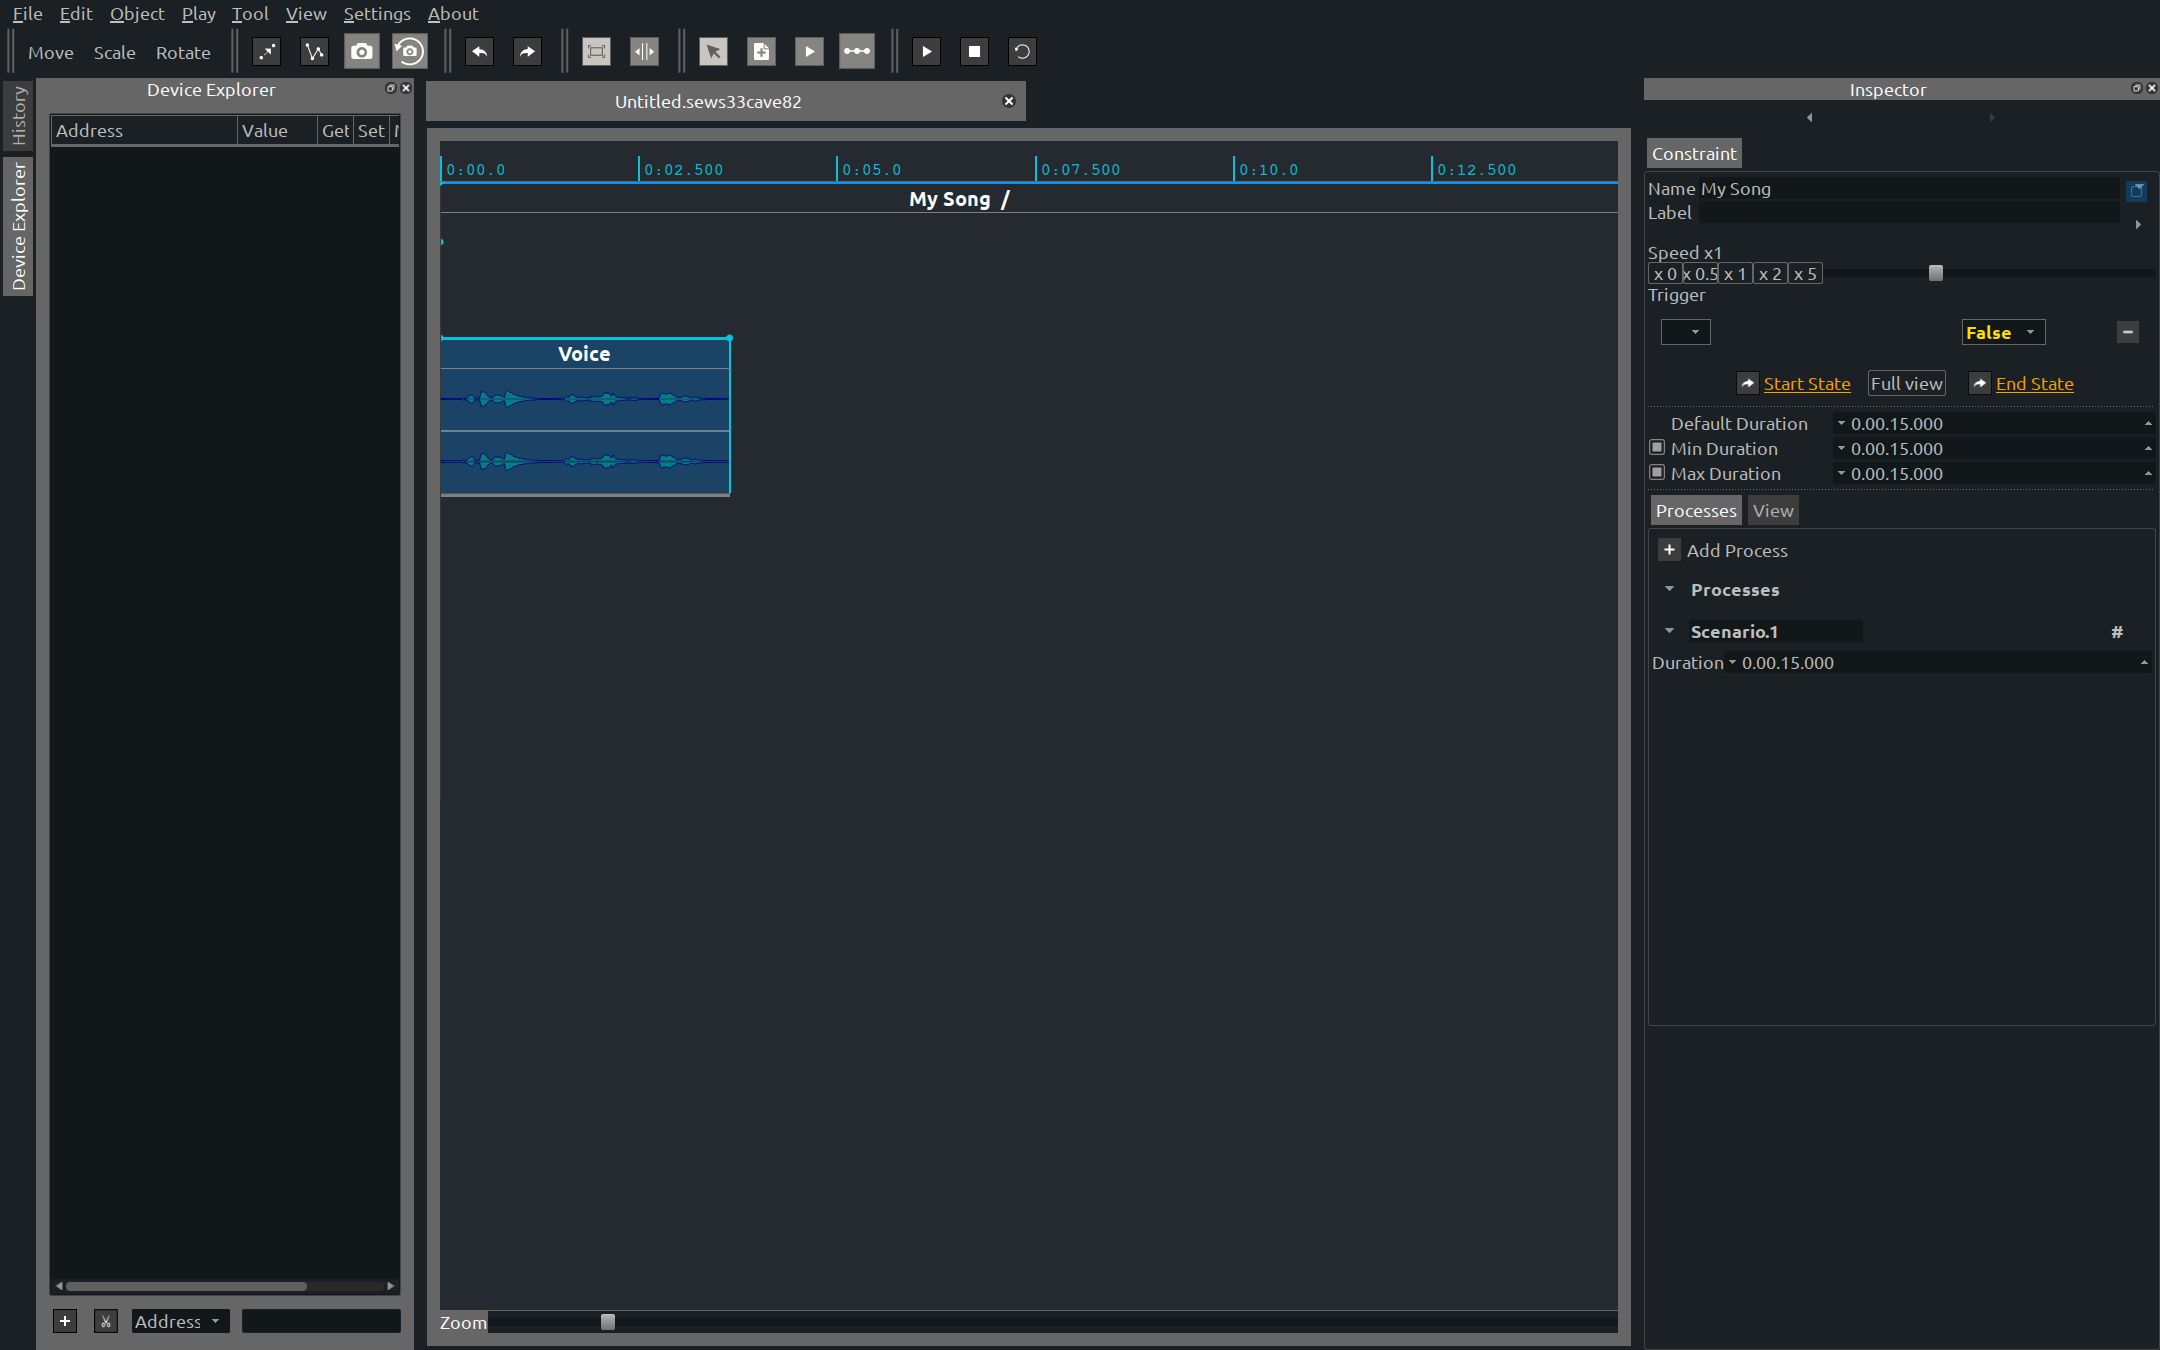
\includegraphics[width=\textwidth]{images/screens/1.png}
    \end{figure}
\end{frame}
\begin{frame} 
    \Large
    \begin{figure}
        \centering
        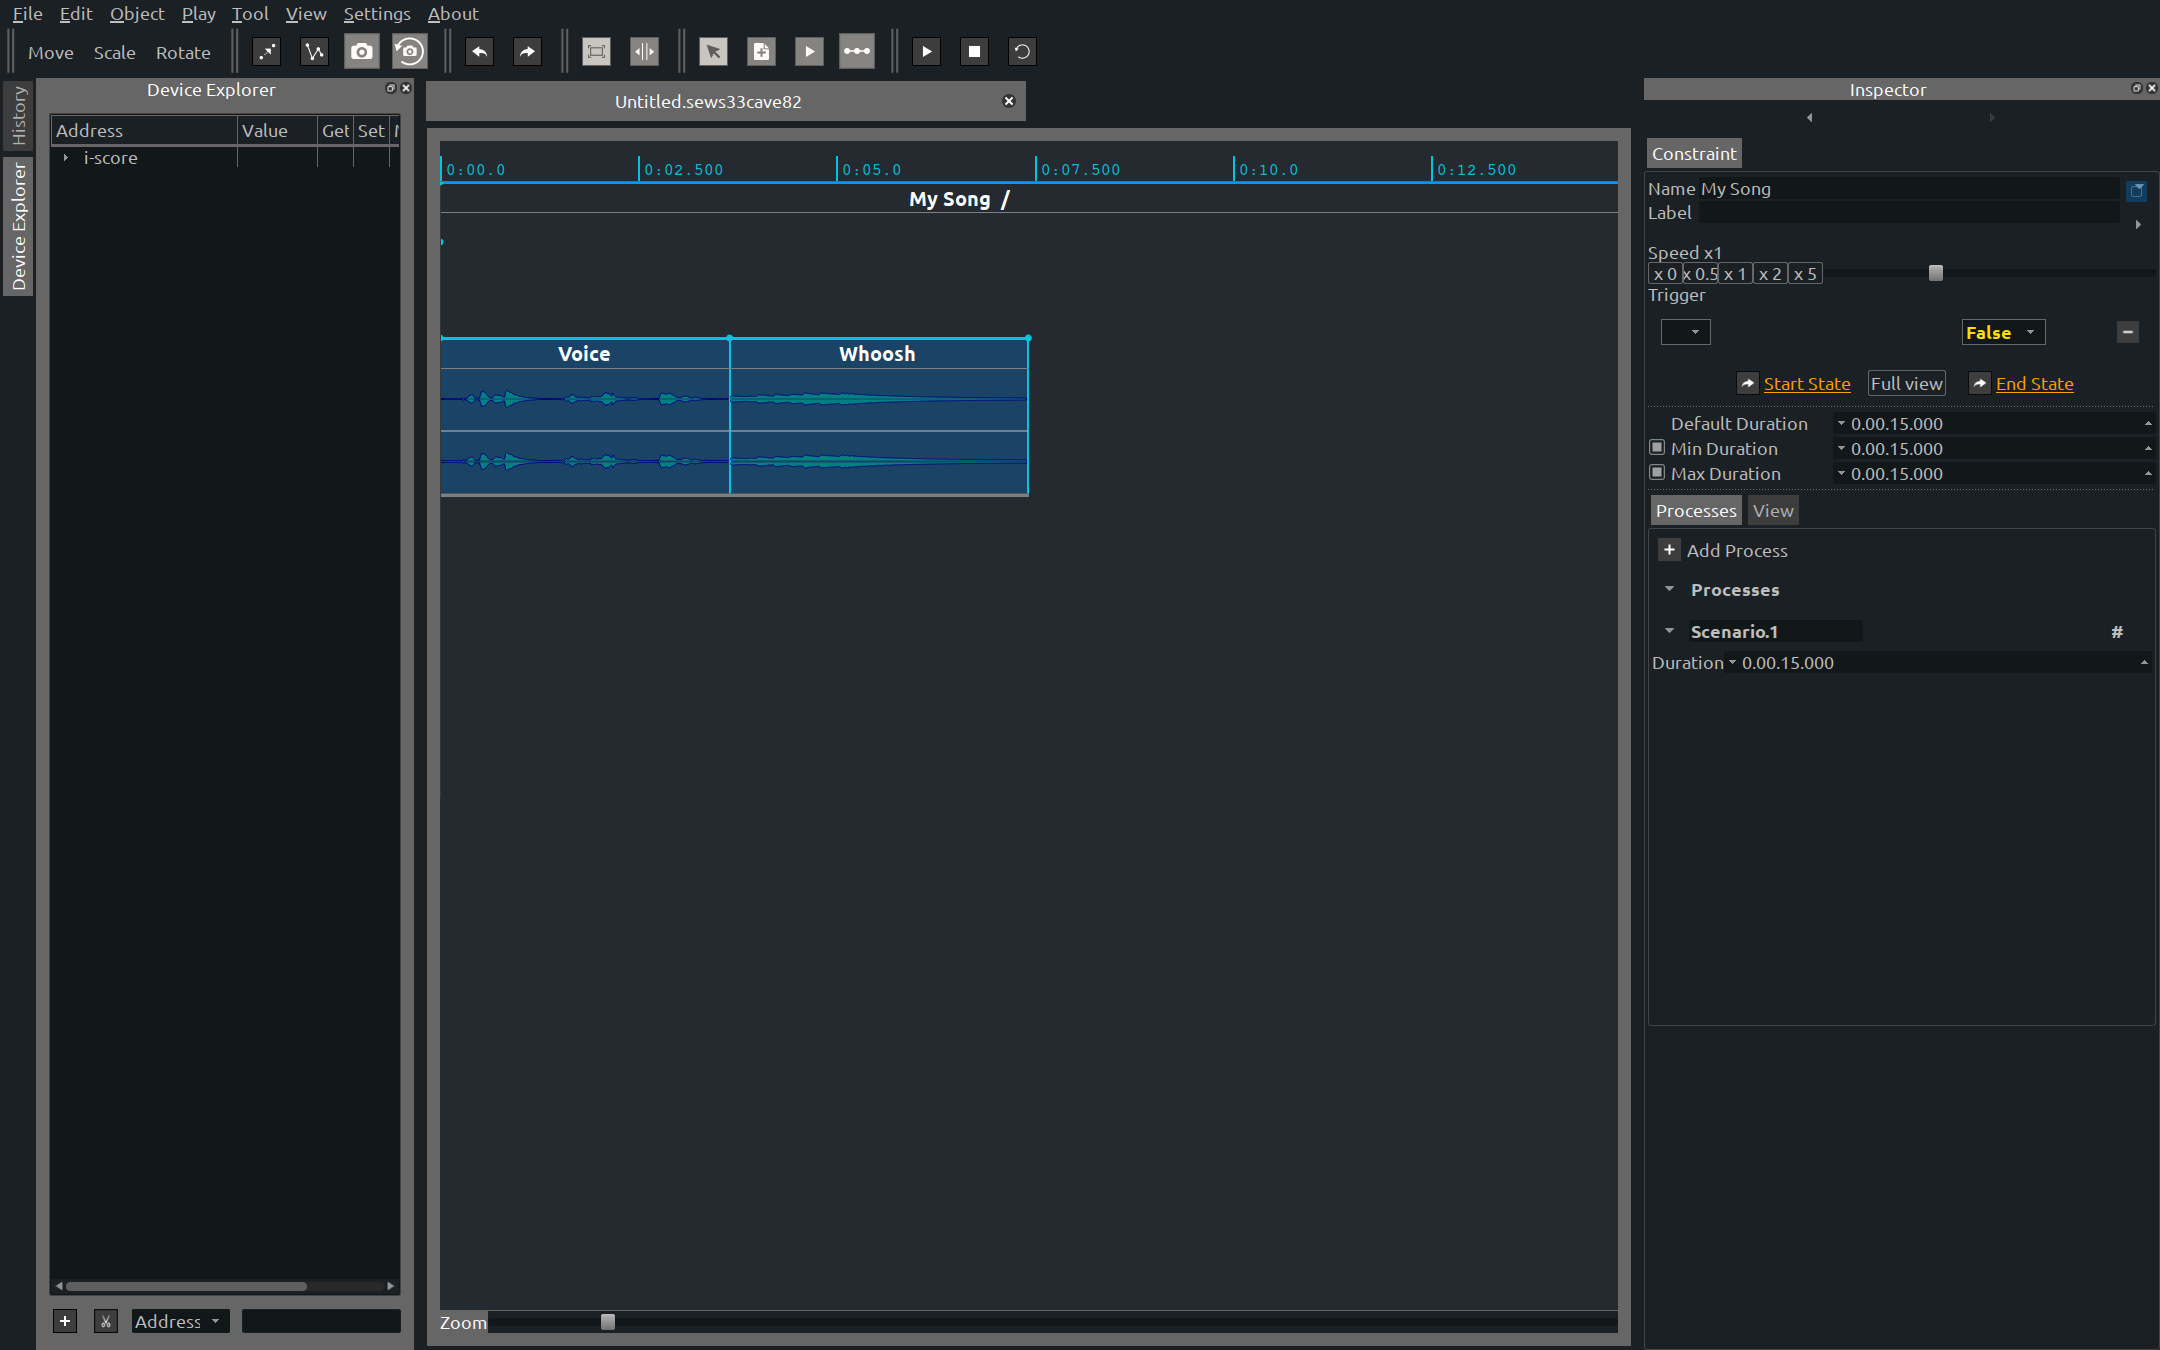
\includegraphics[width=\textwidth]{images/screens/2.png}
    \end{figure}
\end{frame}
\begin{frame} 
    \Large
    \begin{figure}
        \centering
        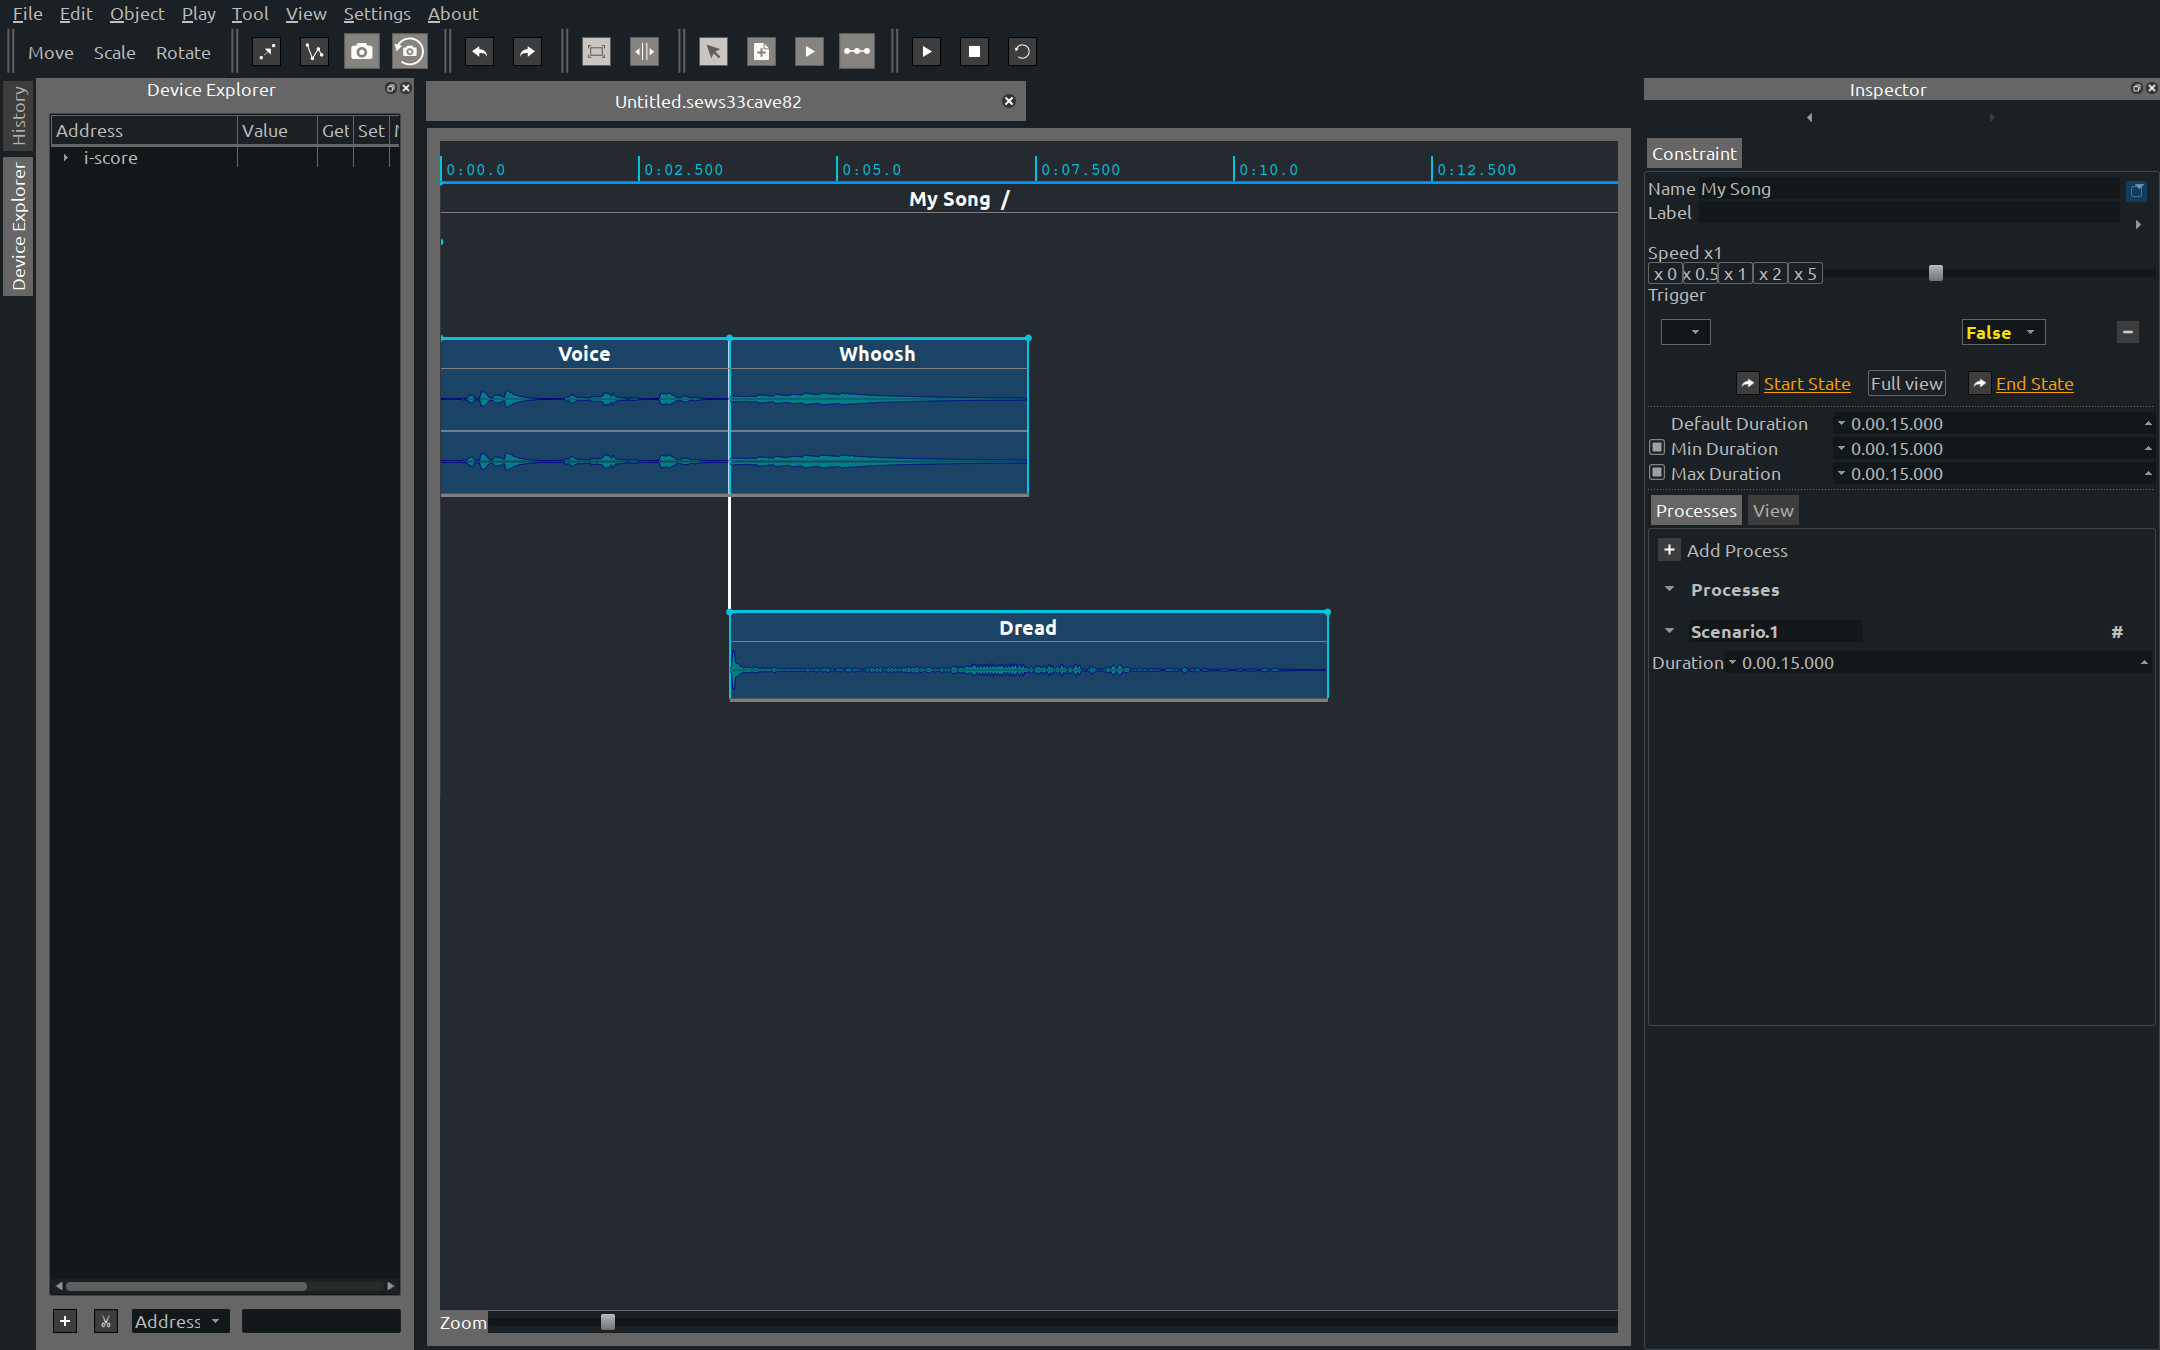
\includegraphics[width=\textwidth]{images/screens/3.png}
    \end{figure}
\end{frame}
\begin{frame} 
    \Large
    \begin{figure}
        \centering
        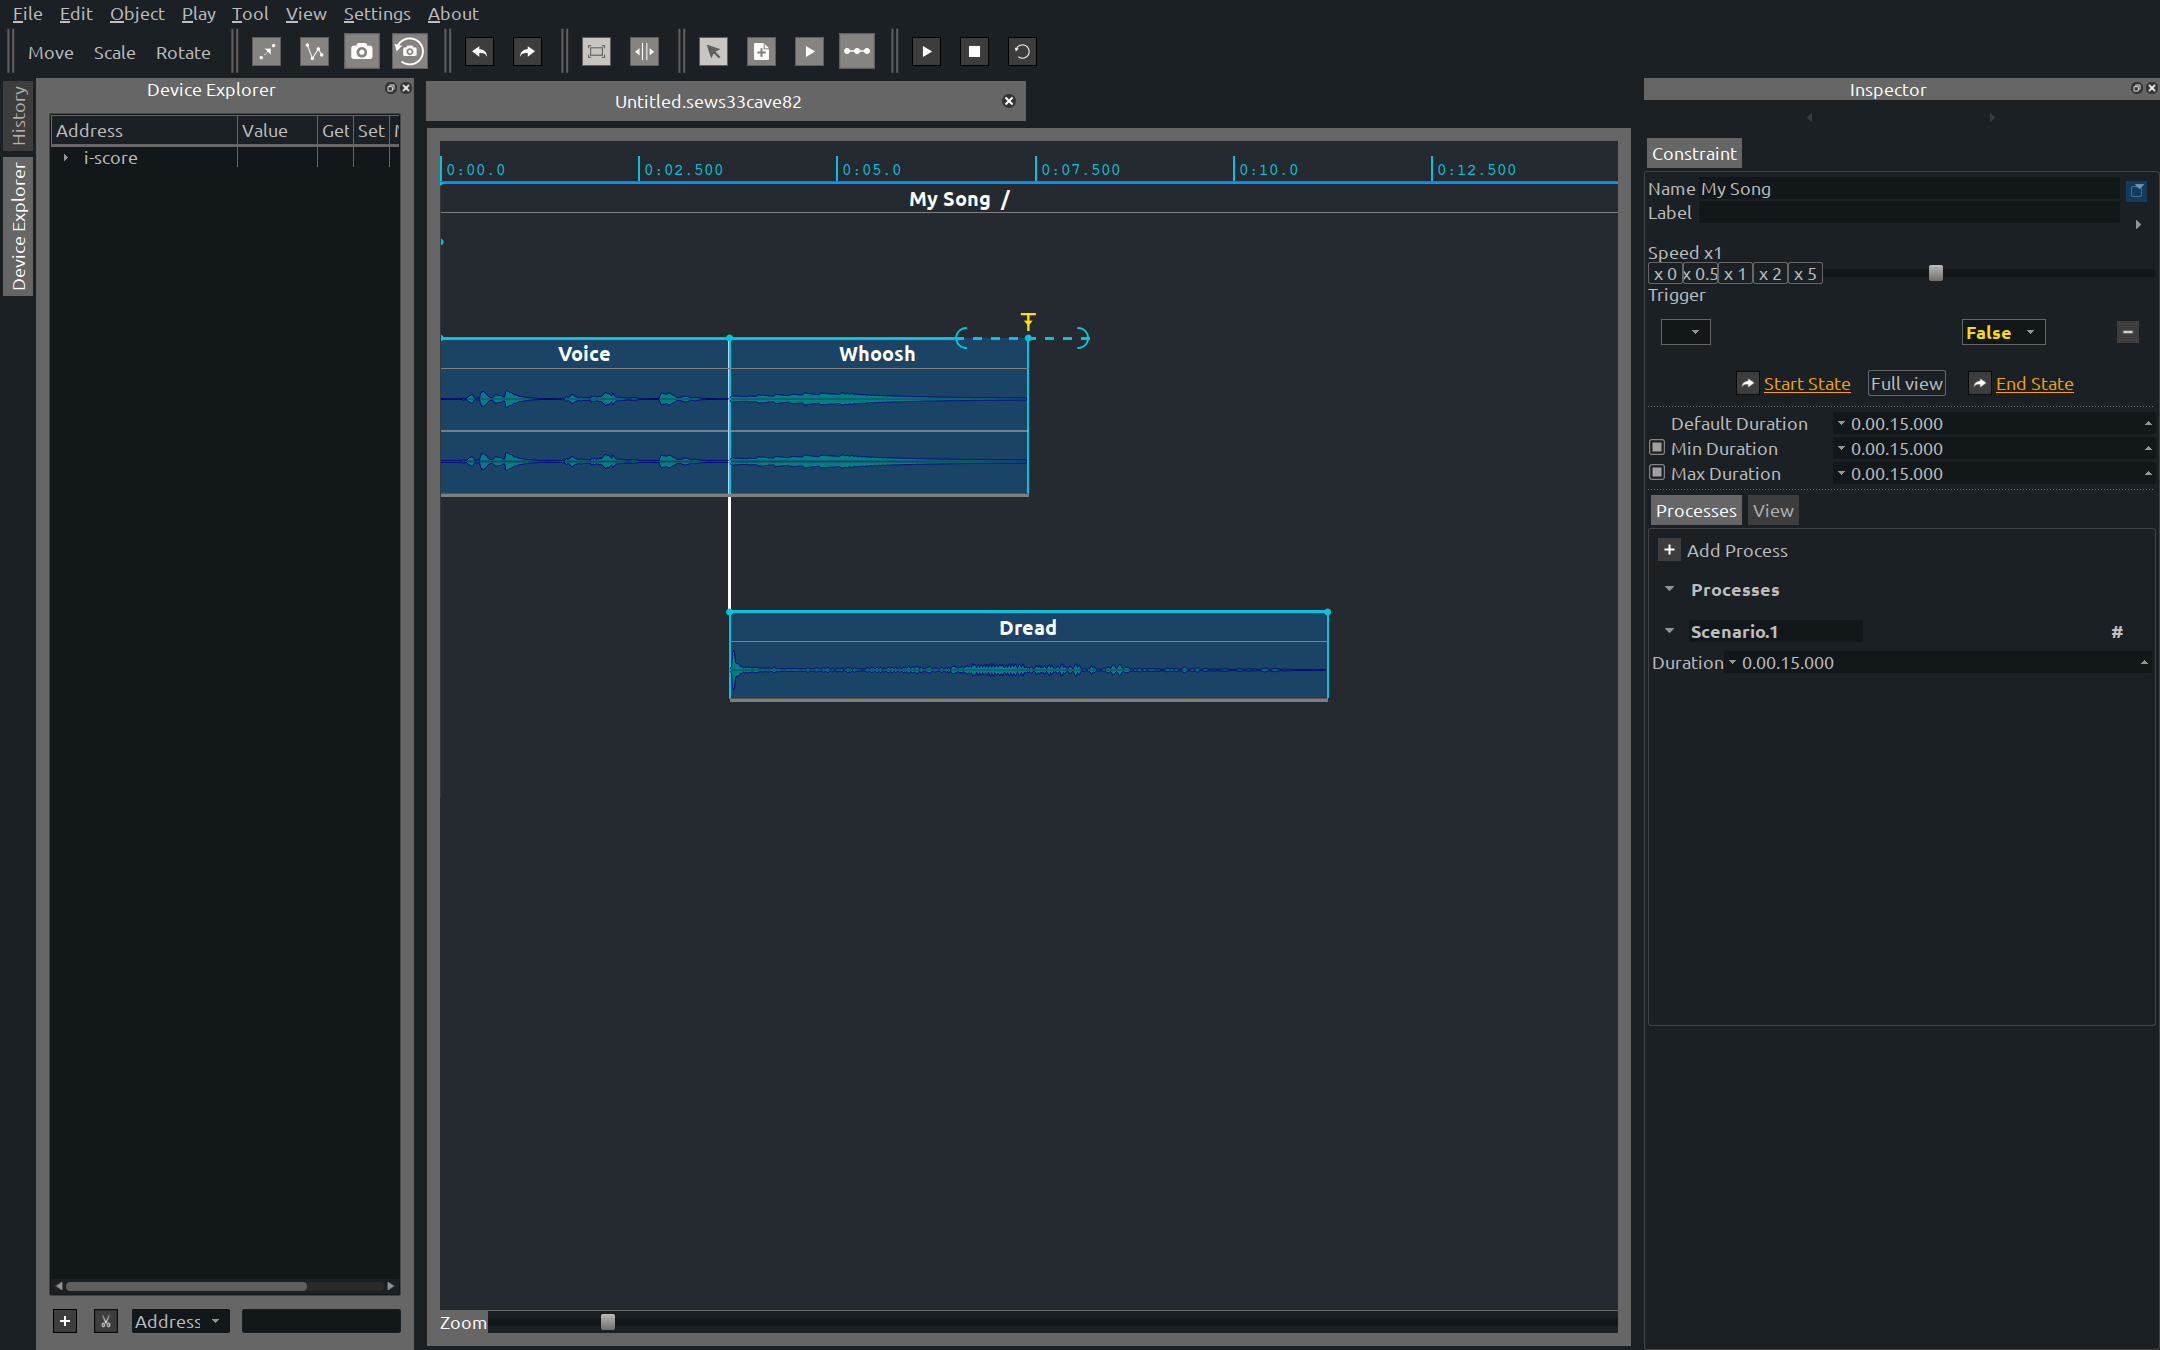
\includegraphics[width=\textwidth]{images/screens/4.png}
    \end{figure}
\end{frame}
\begin{frame} 
    \Large
    \begin{figure}
        \centering
        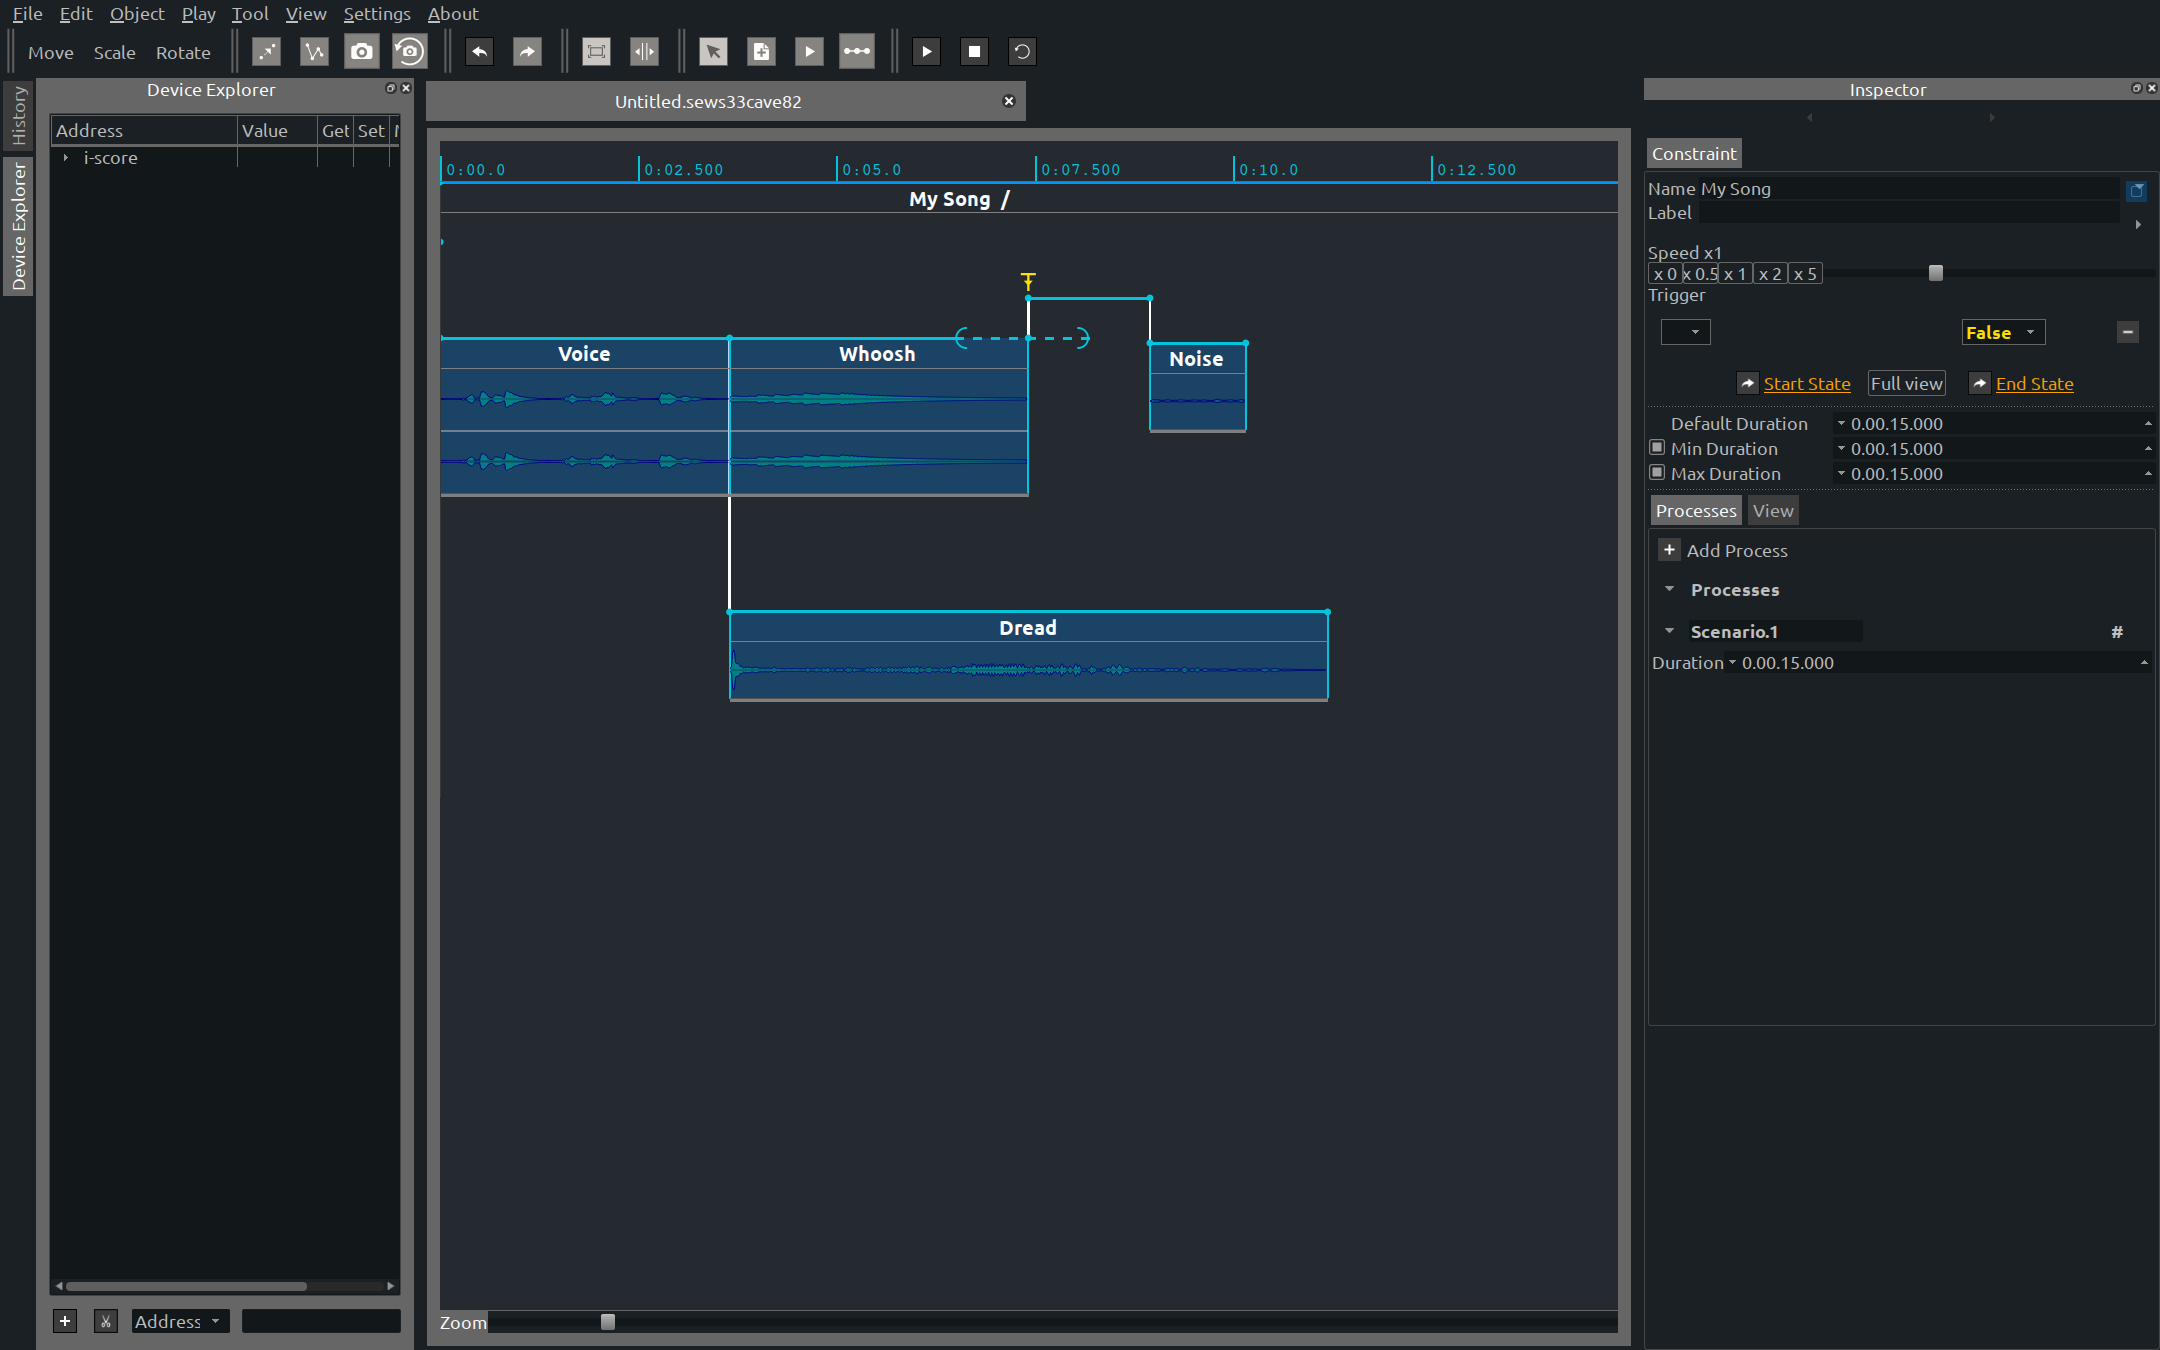
\includegraphics[width=\textwidth]{images/screens/5.png}
    \end{figure}
\end{frame}
\begin{frame} 
    \Large
    \begin{figure}
        \centering
        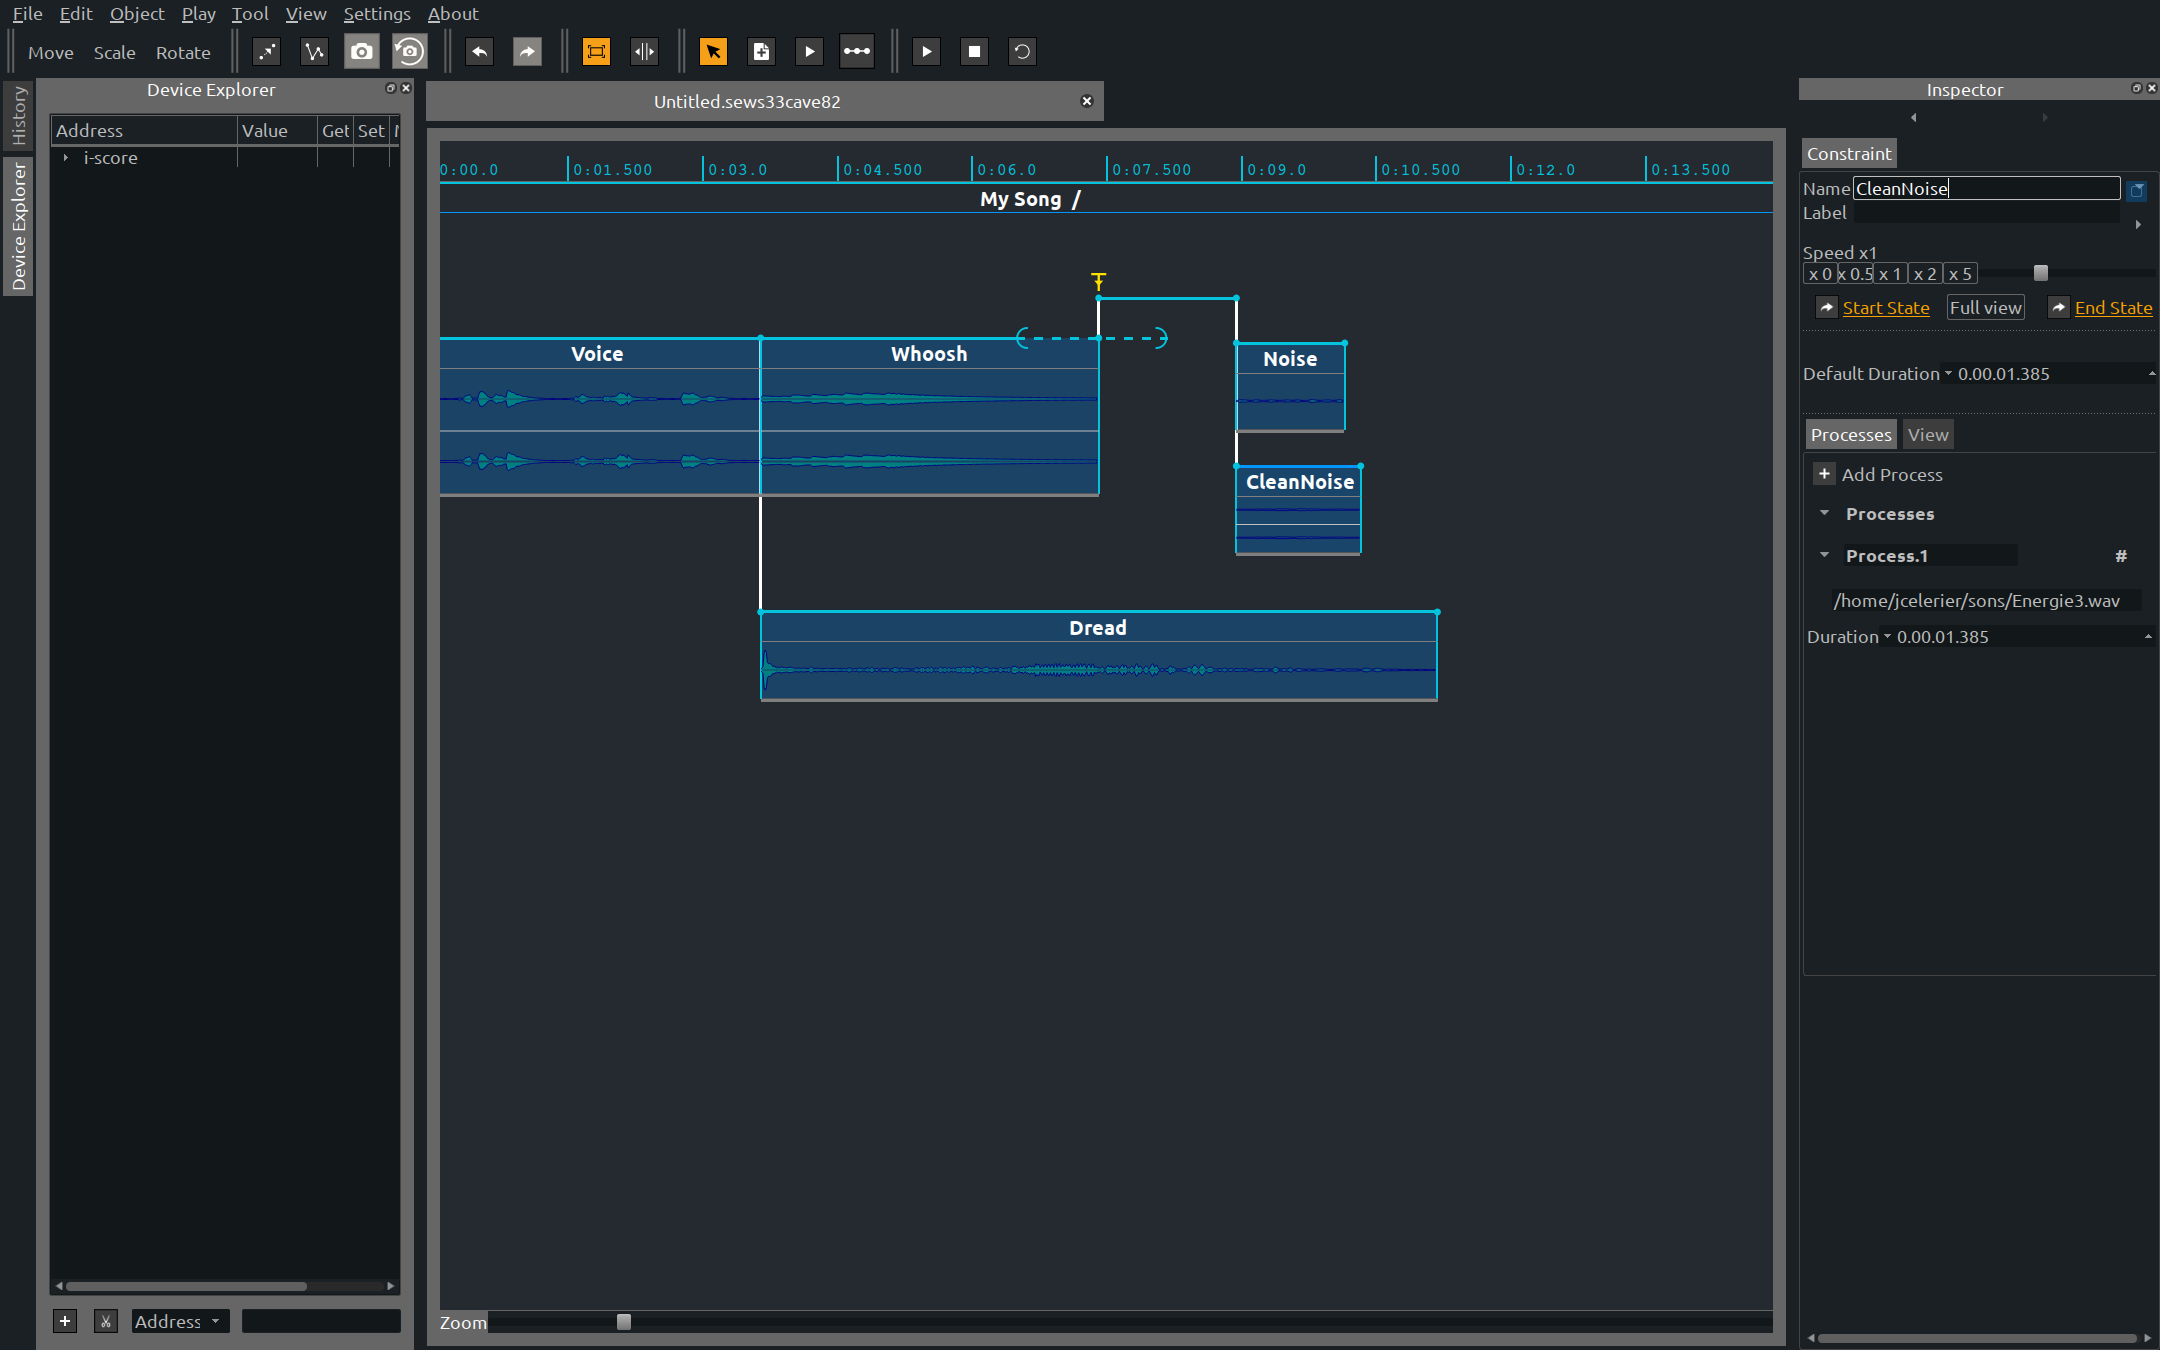
\includegraphics[width=\textwidth]{images/screens/6.png}
    \end{figure}
\end{frame}
\begin{frame} 
    \Large
    \begin{figure}
        \centering
        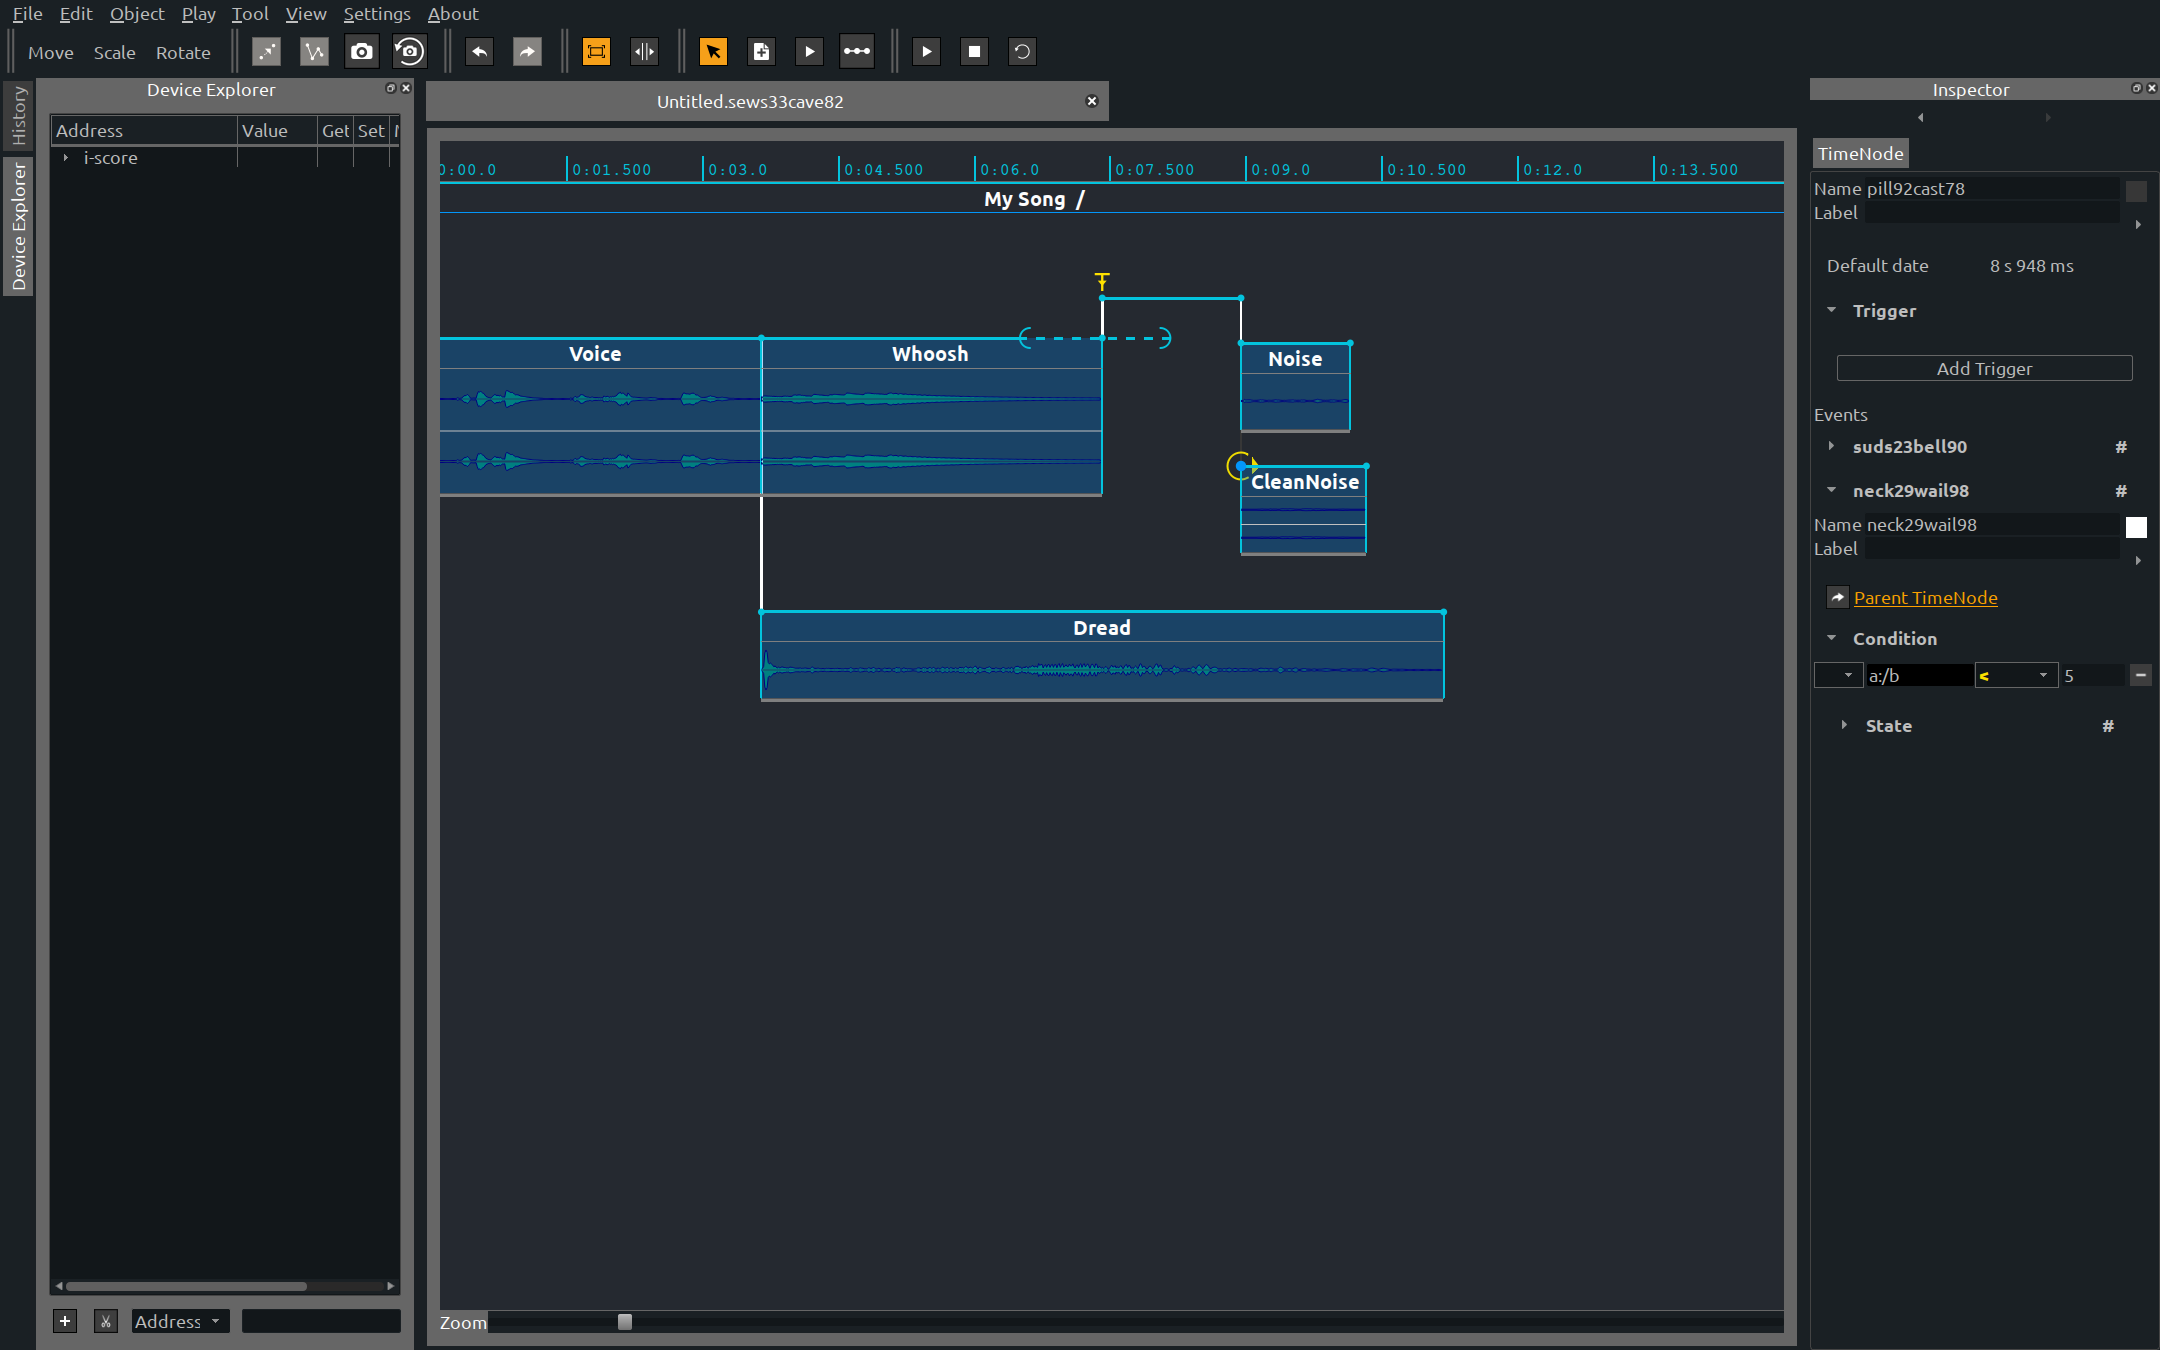
\includegraphics[width=\textwidth]{images/screens/7.png}
    \end{figure}
\end{frame}
\begin{frame} 
    \Large
    \begin{figure}
        \centering
        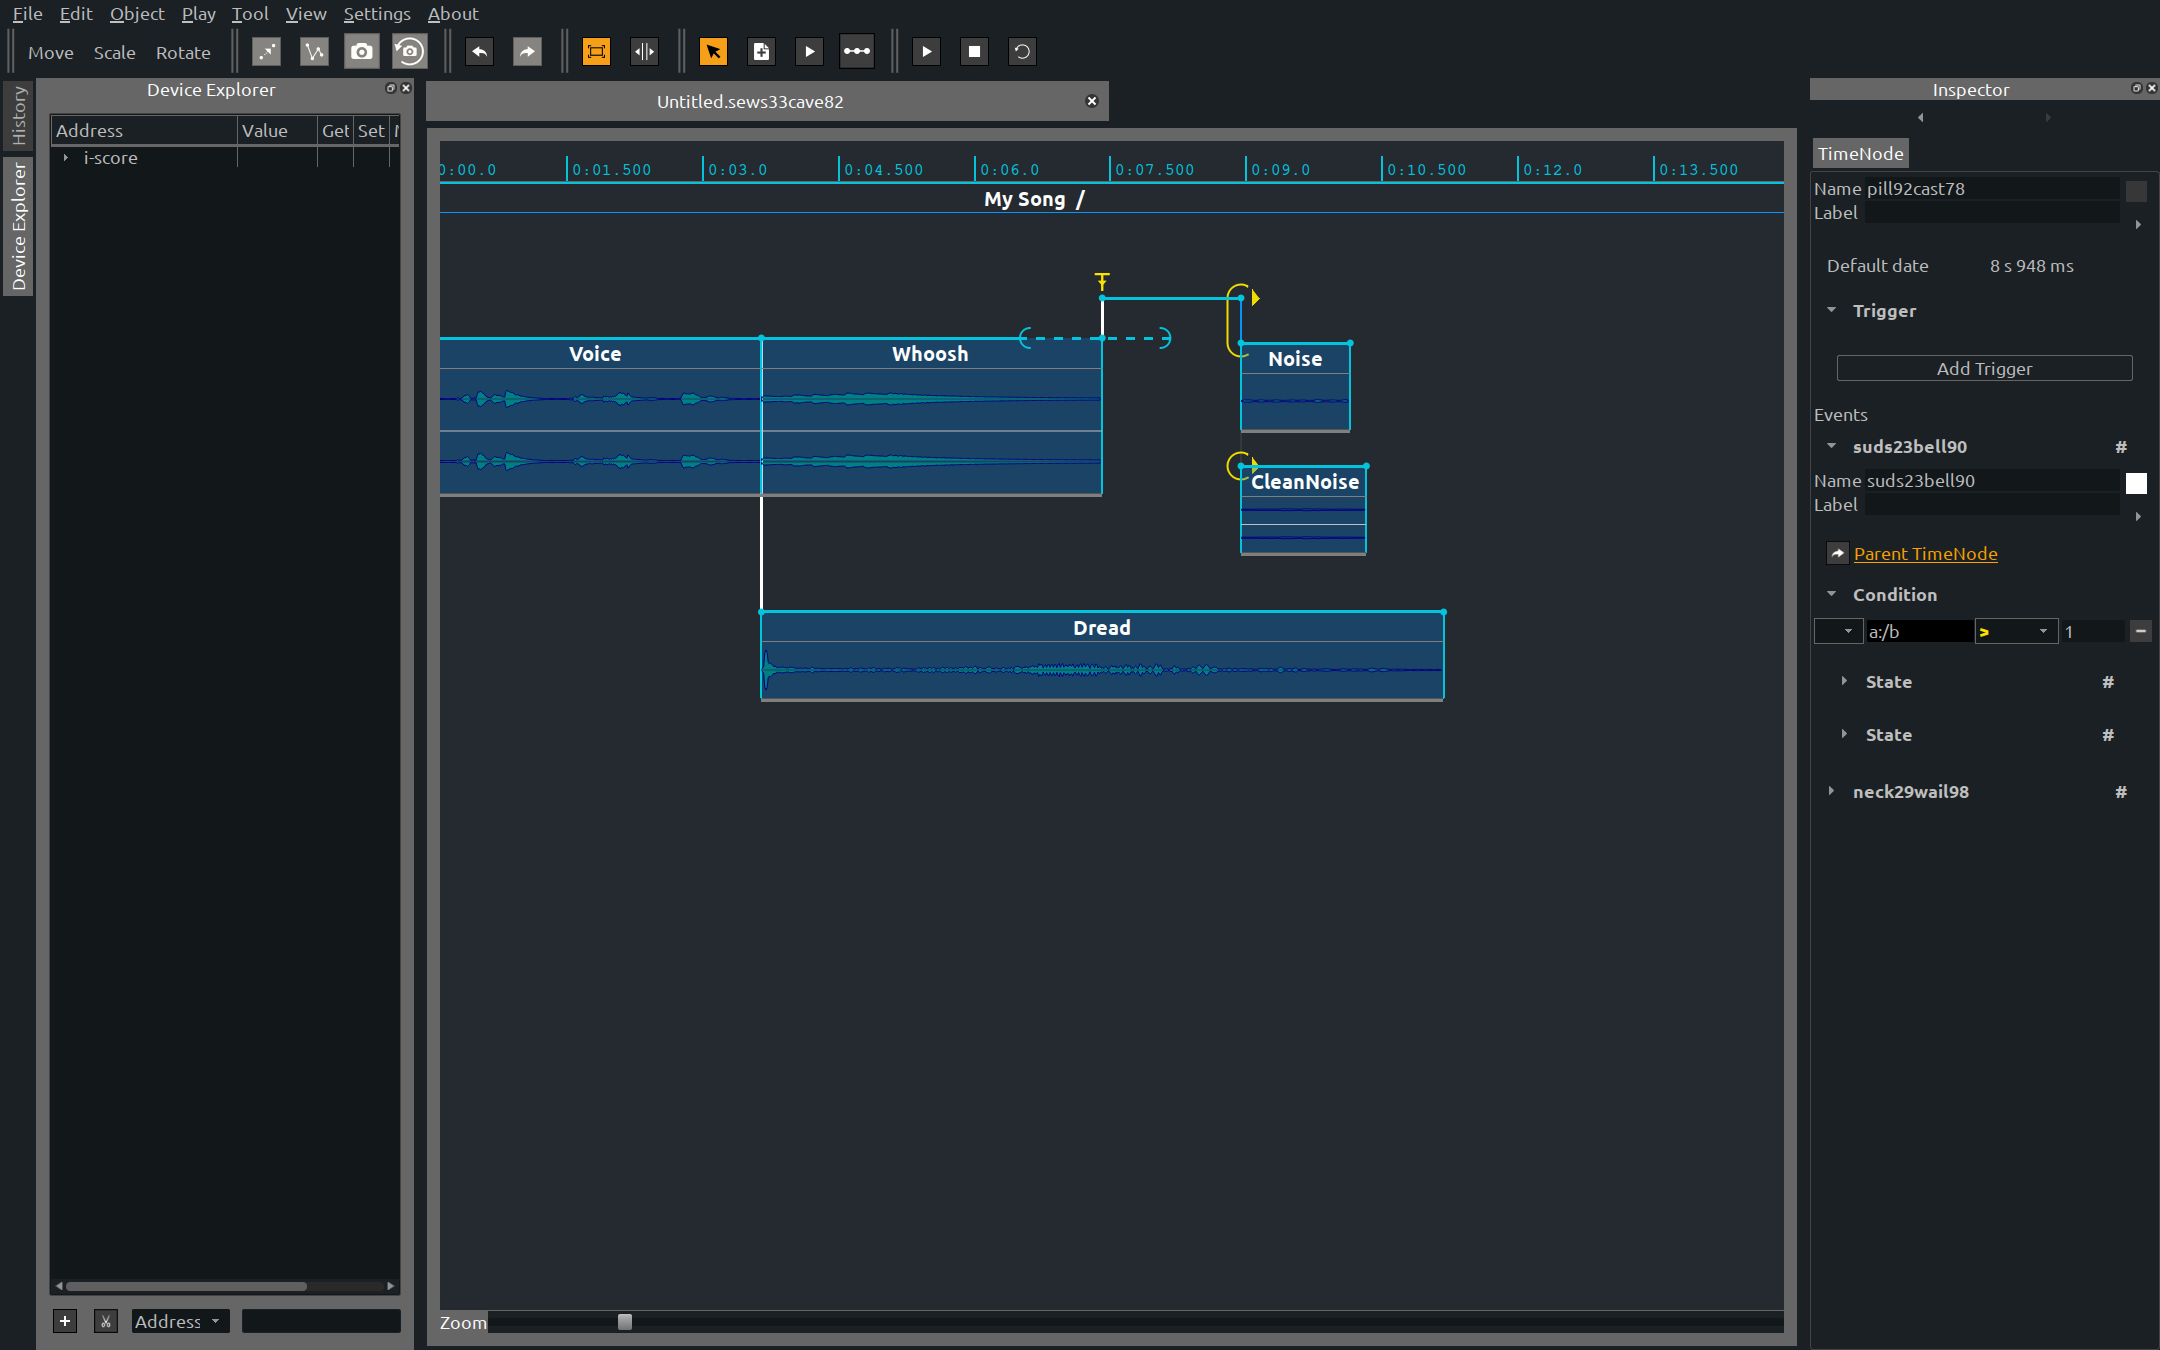
\includegraphics[width=\textwidth]{images/screens/8.png}
    \end{figure}
\end{frame}
\begin{frame} 
    \Large
    \begin{figure}
        \centering
        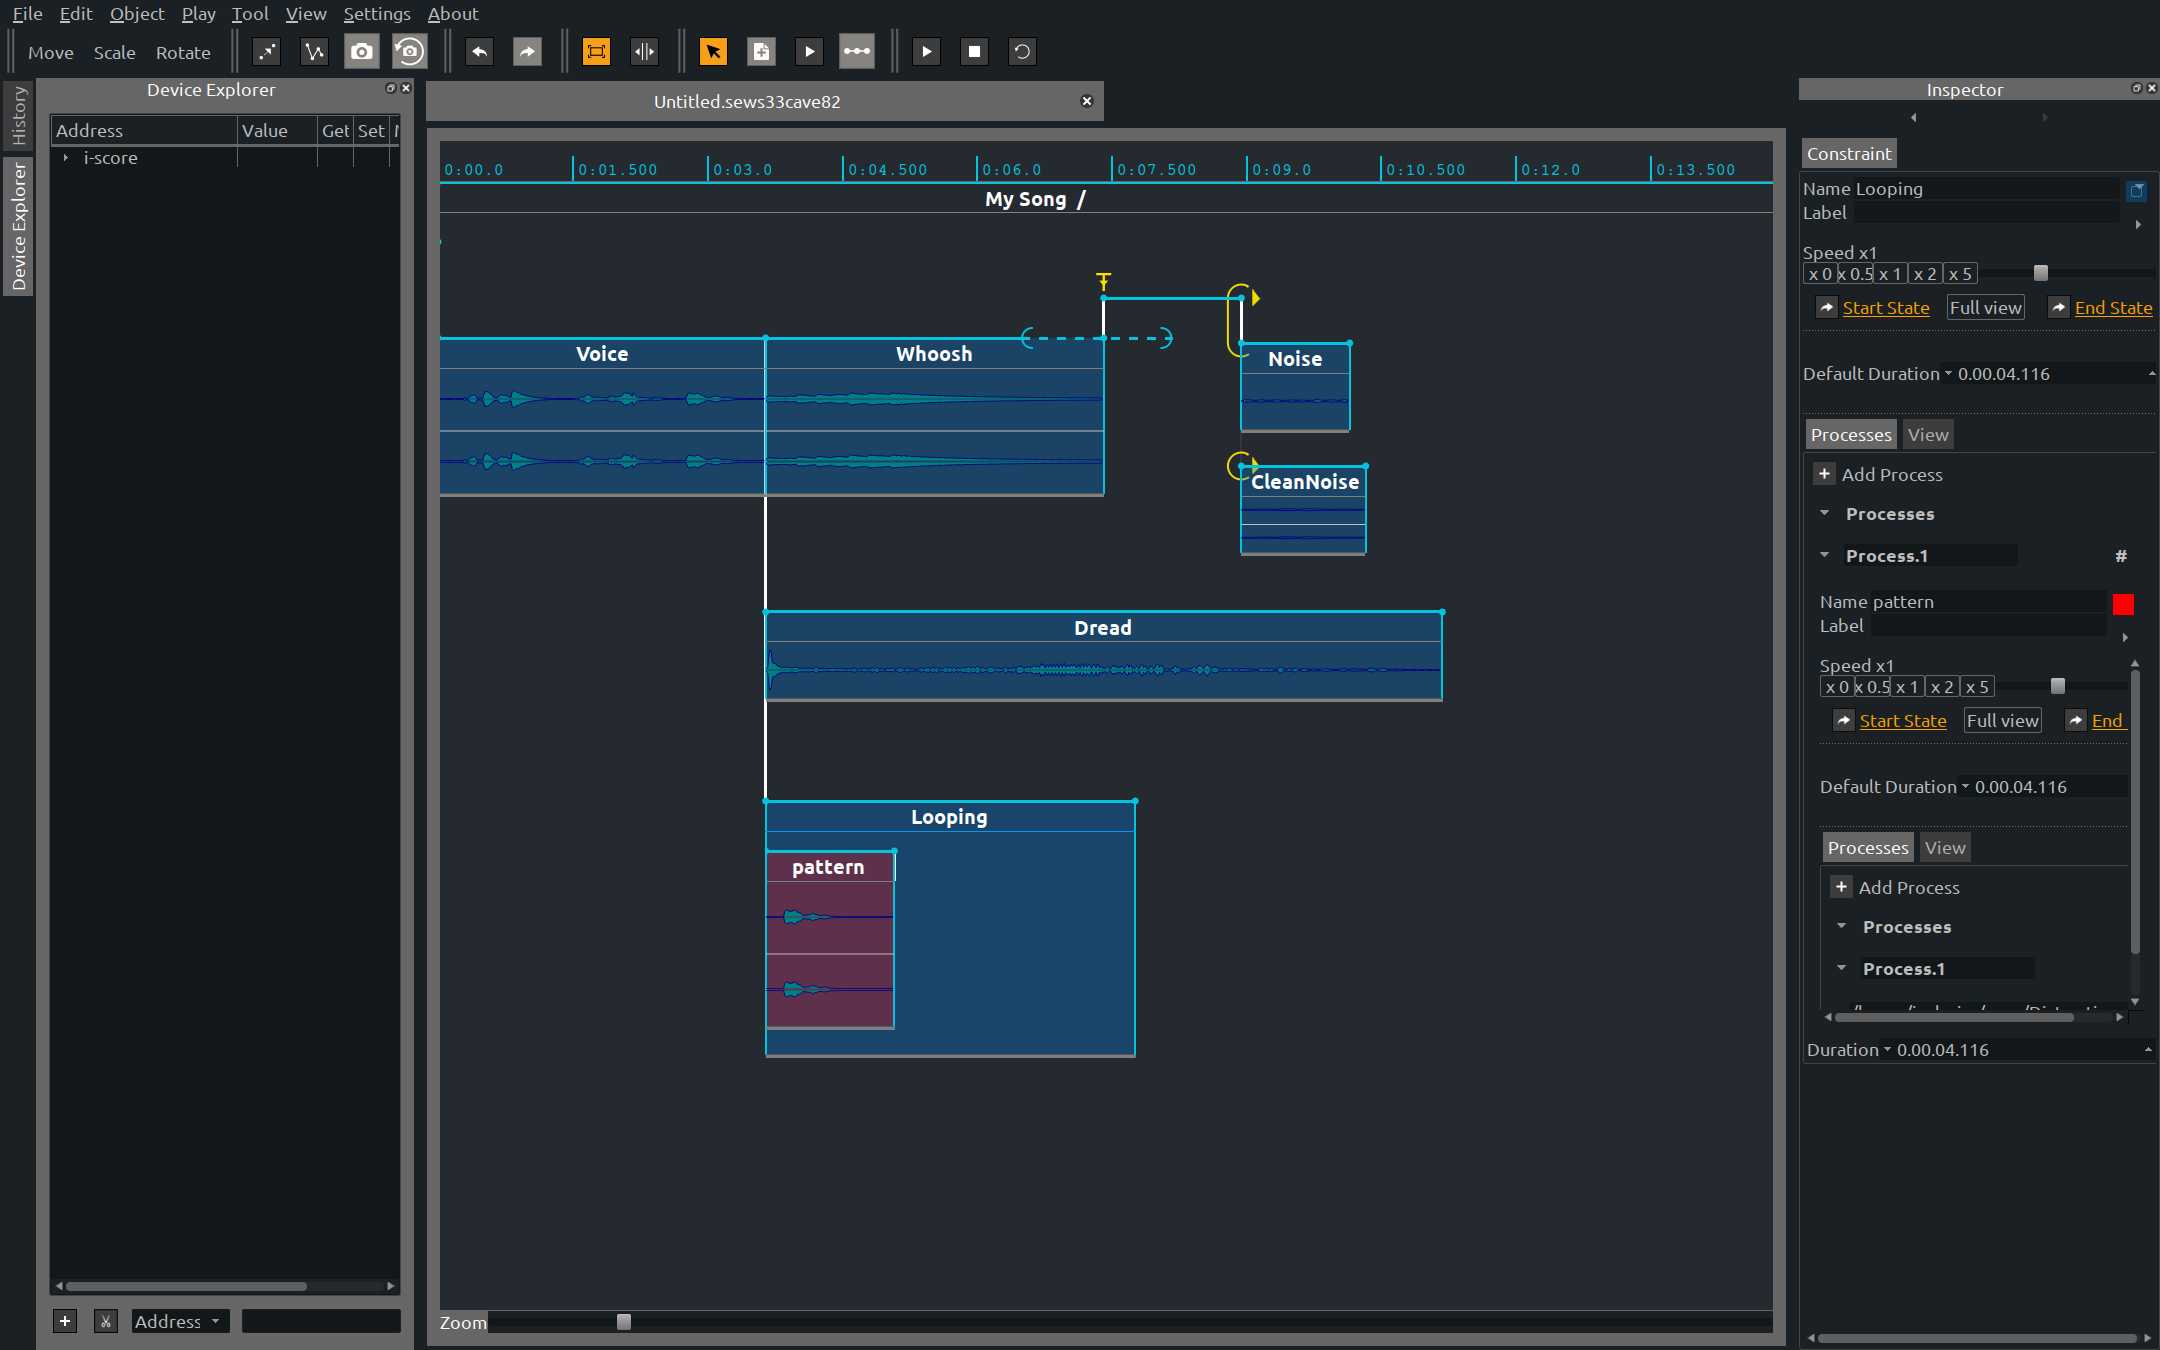
\includegraphics[width=\textwidth]{images/screens/9.png}
    \end{figure}
\end{frame}
\begin{frame} 
    \Large
    \begin{figure}
        \centering
        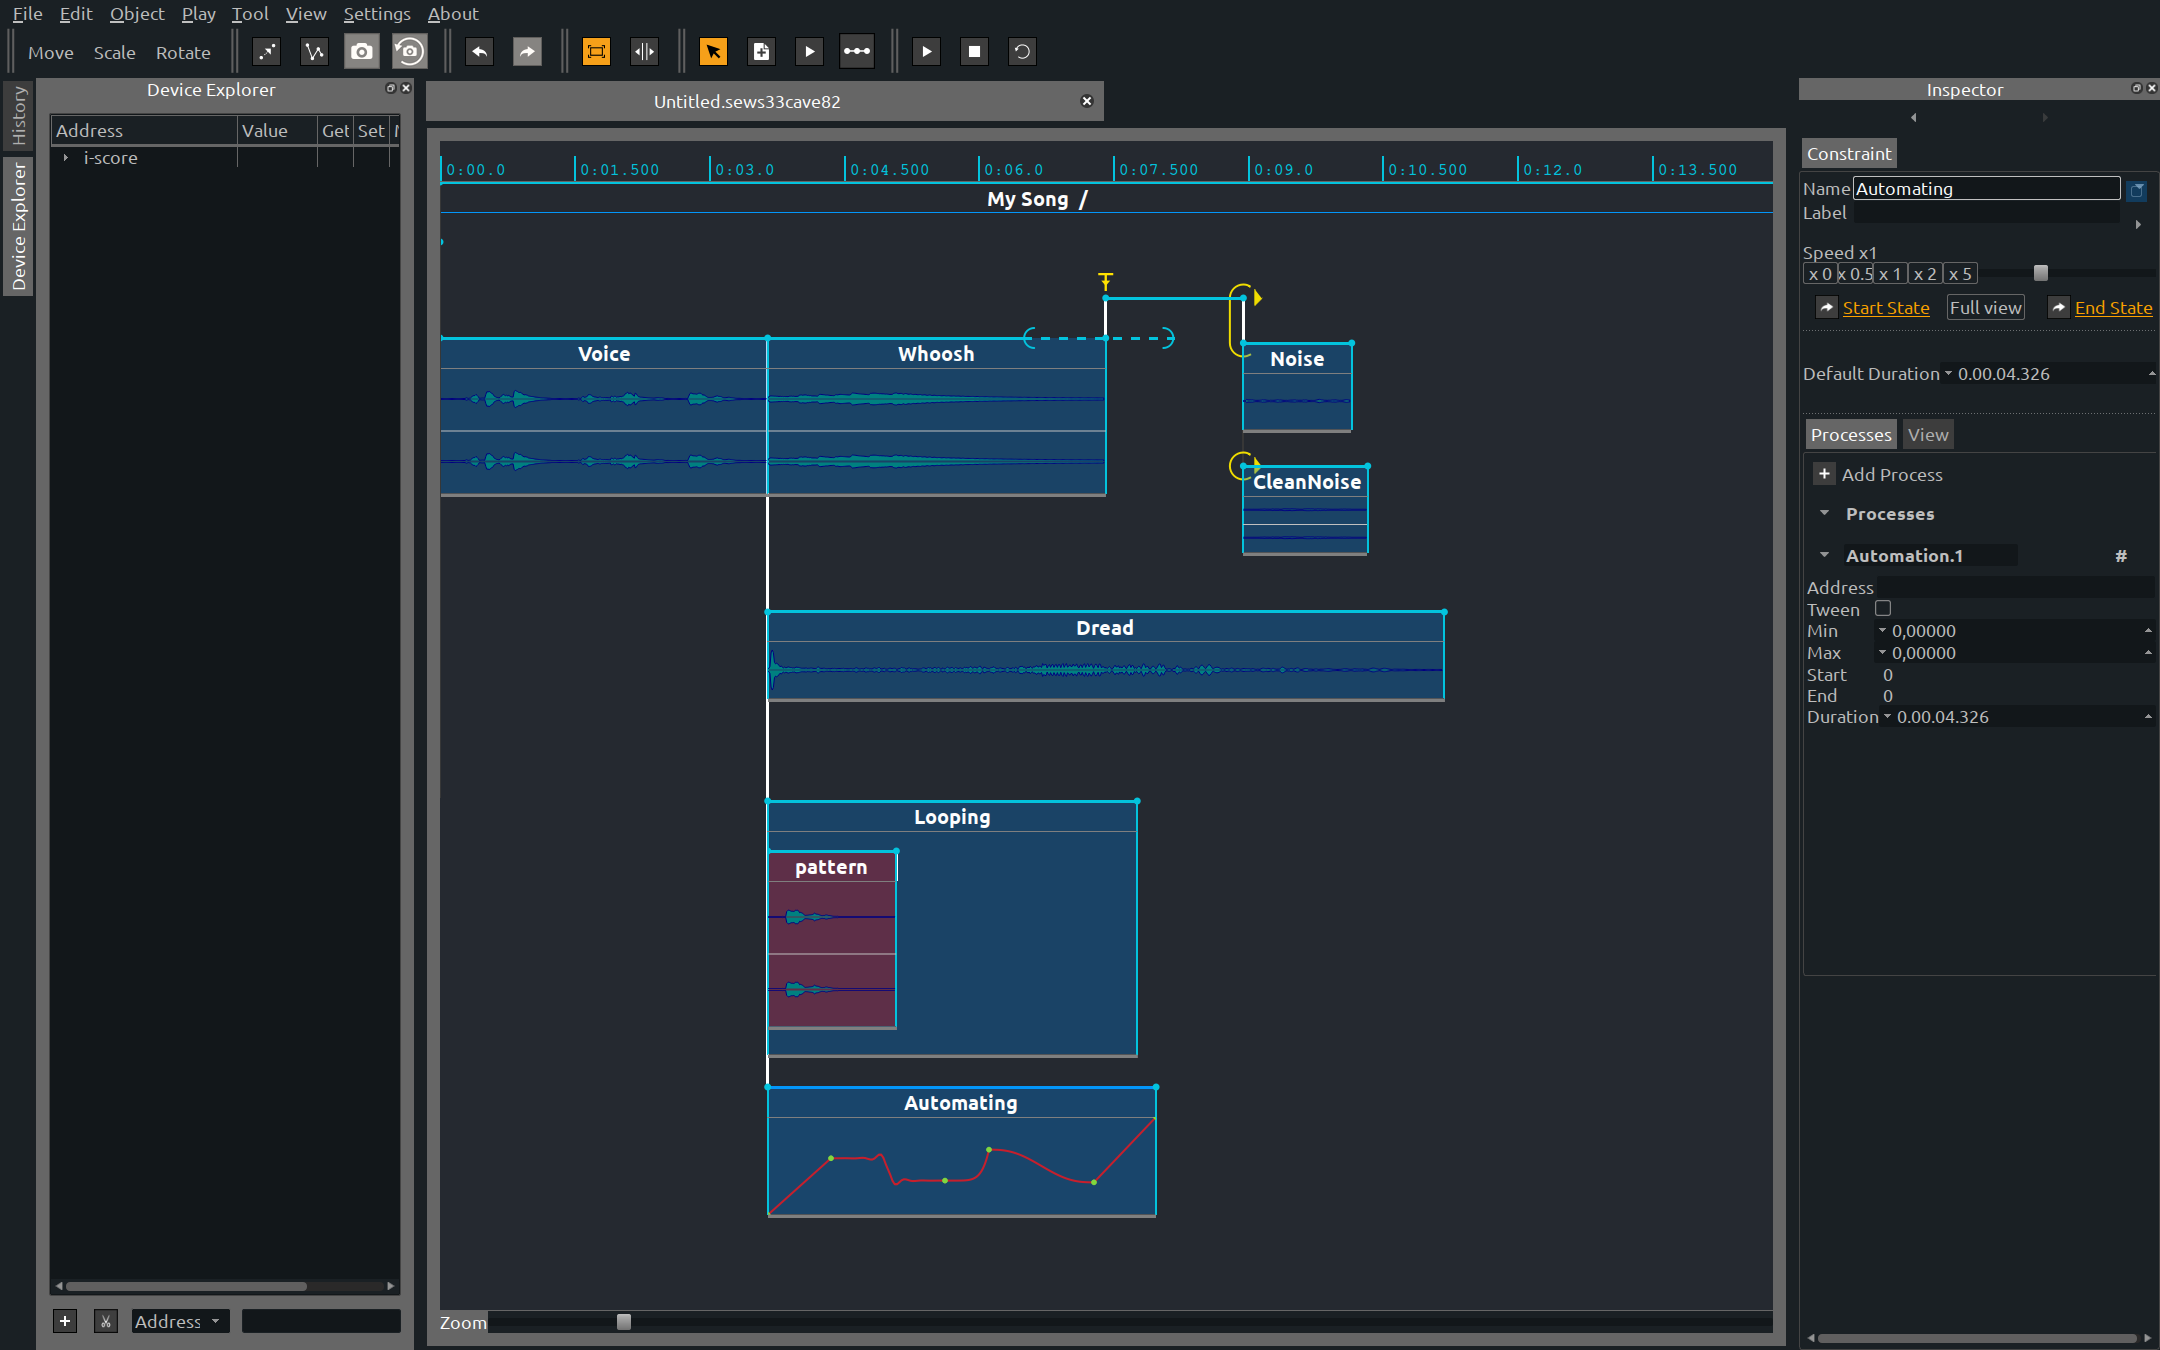
\includegraphics[width=\textwidth]{images/screens/10.png}
    \end{figure}
\end{frame}
\begin{frame} 
    \Large
    \begin{figure}
        \centering
        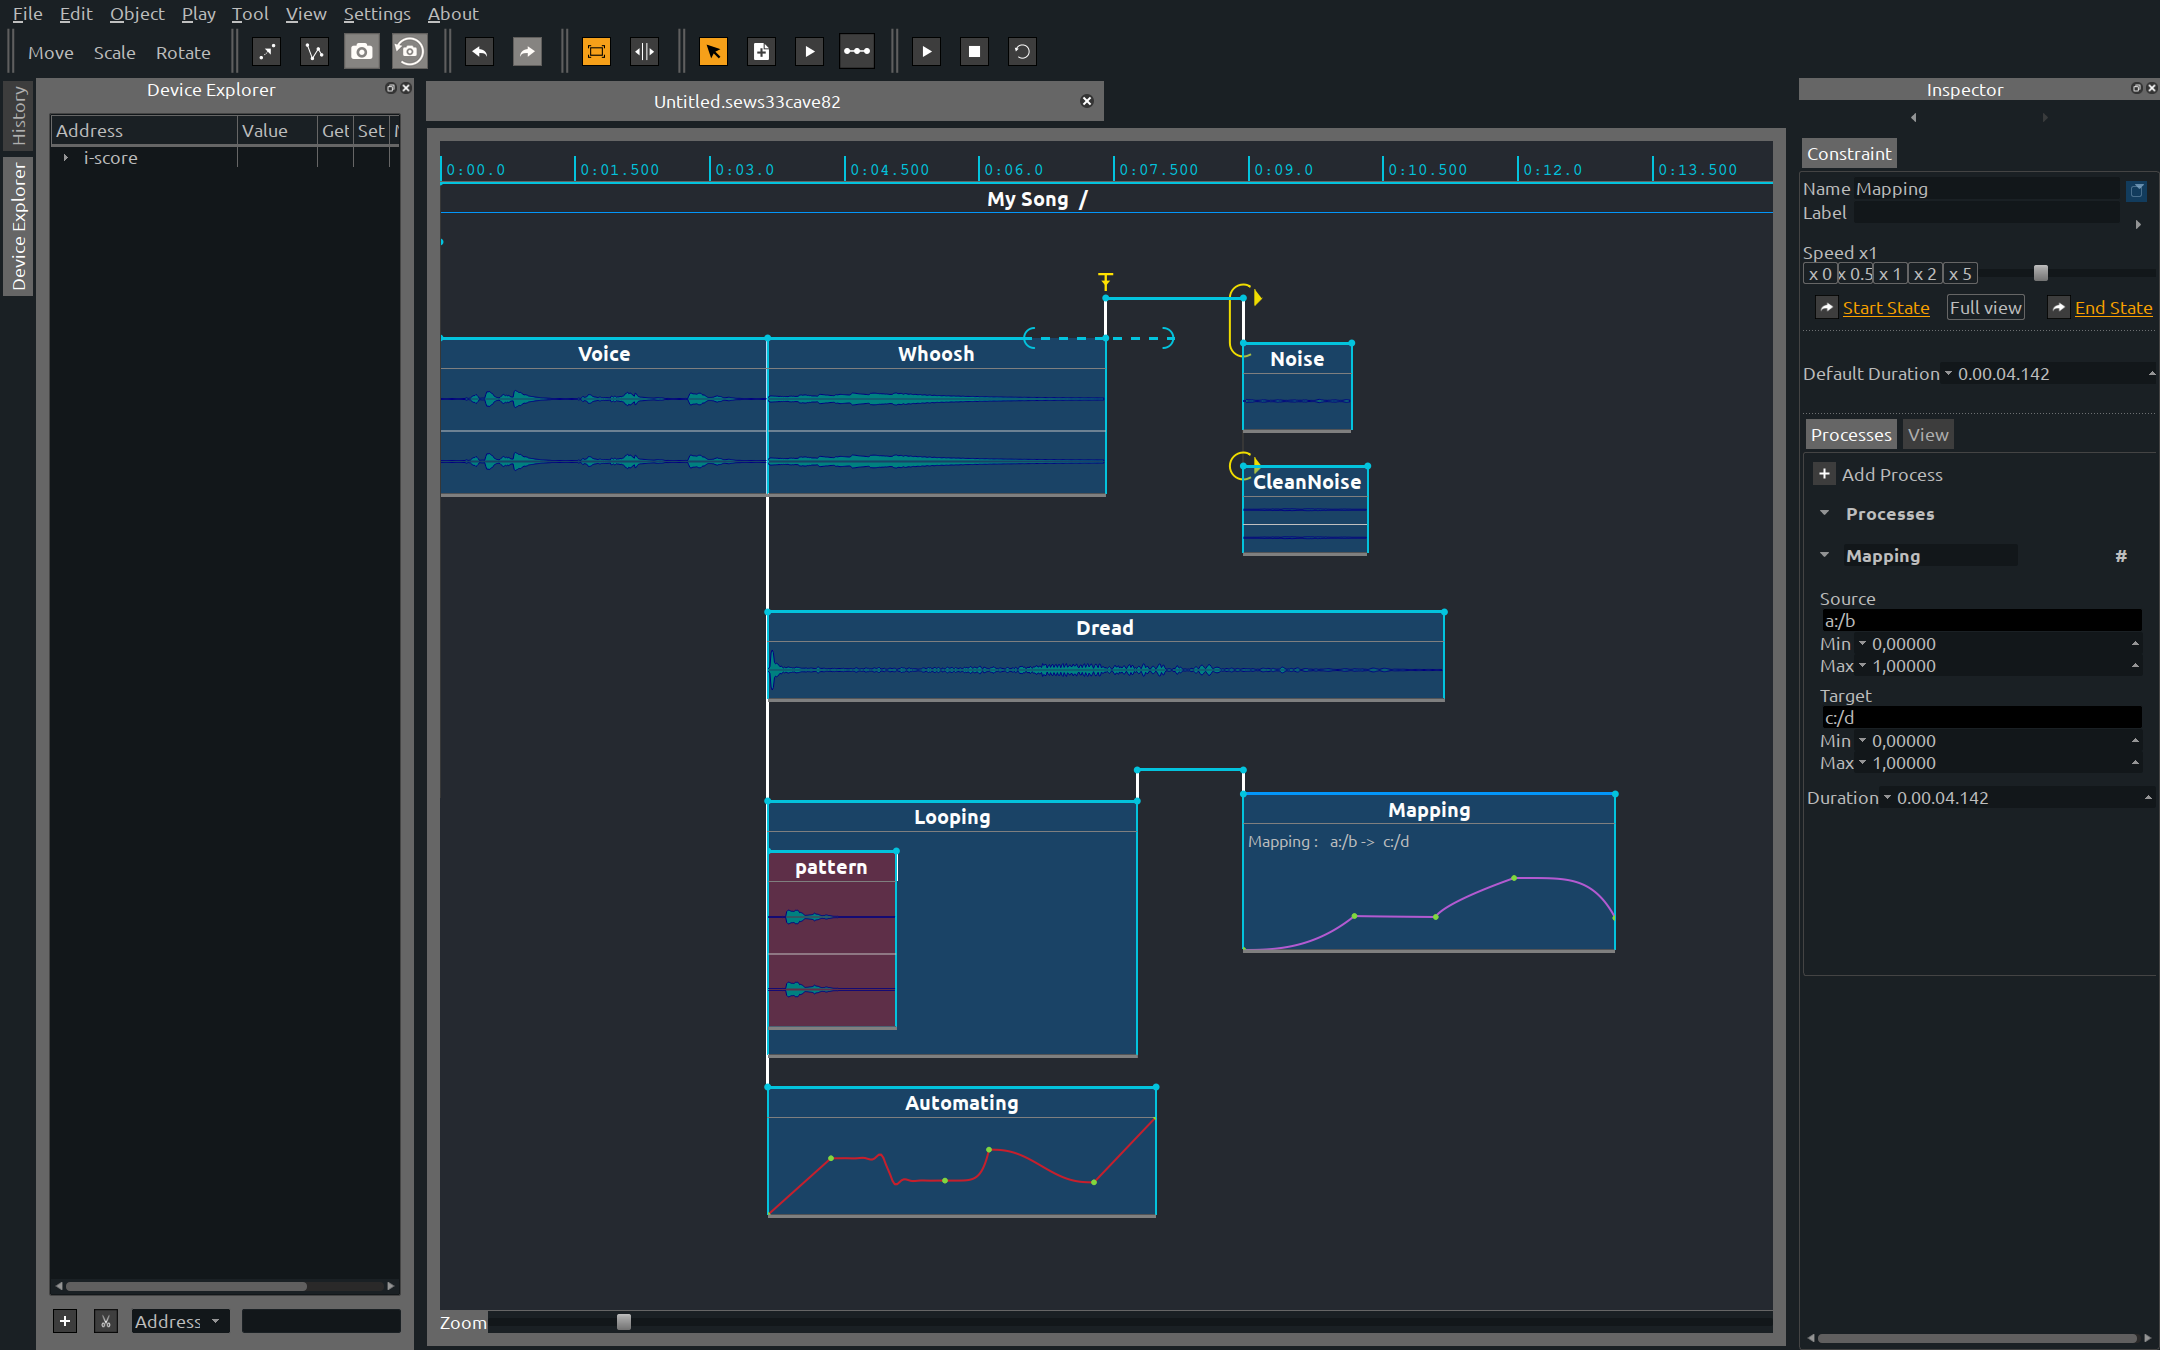
\includegraphics[width=\textwidth]{images/screens/11.png}
    \end{figure}
\end{frame}
\begin{frame} 
    \Large
    \begin{figure}
        \centering
        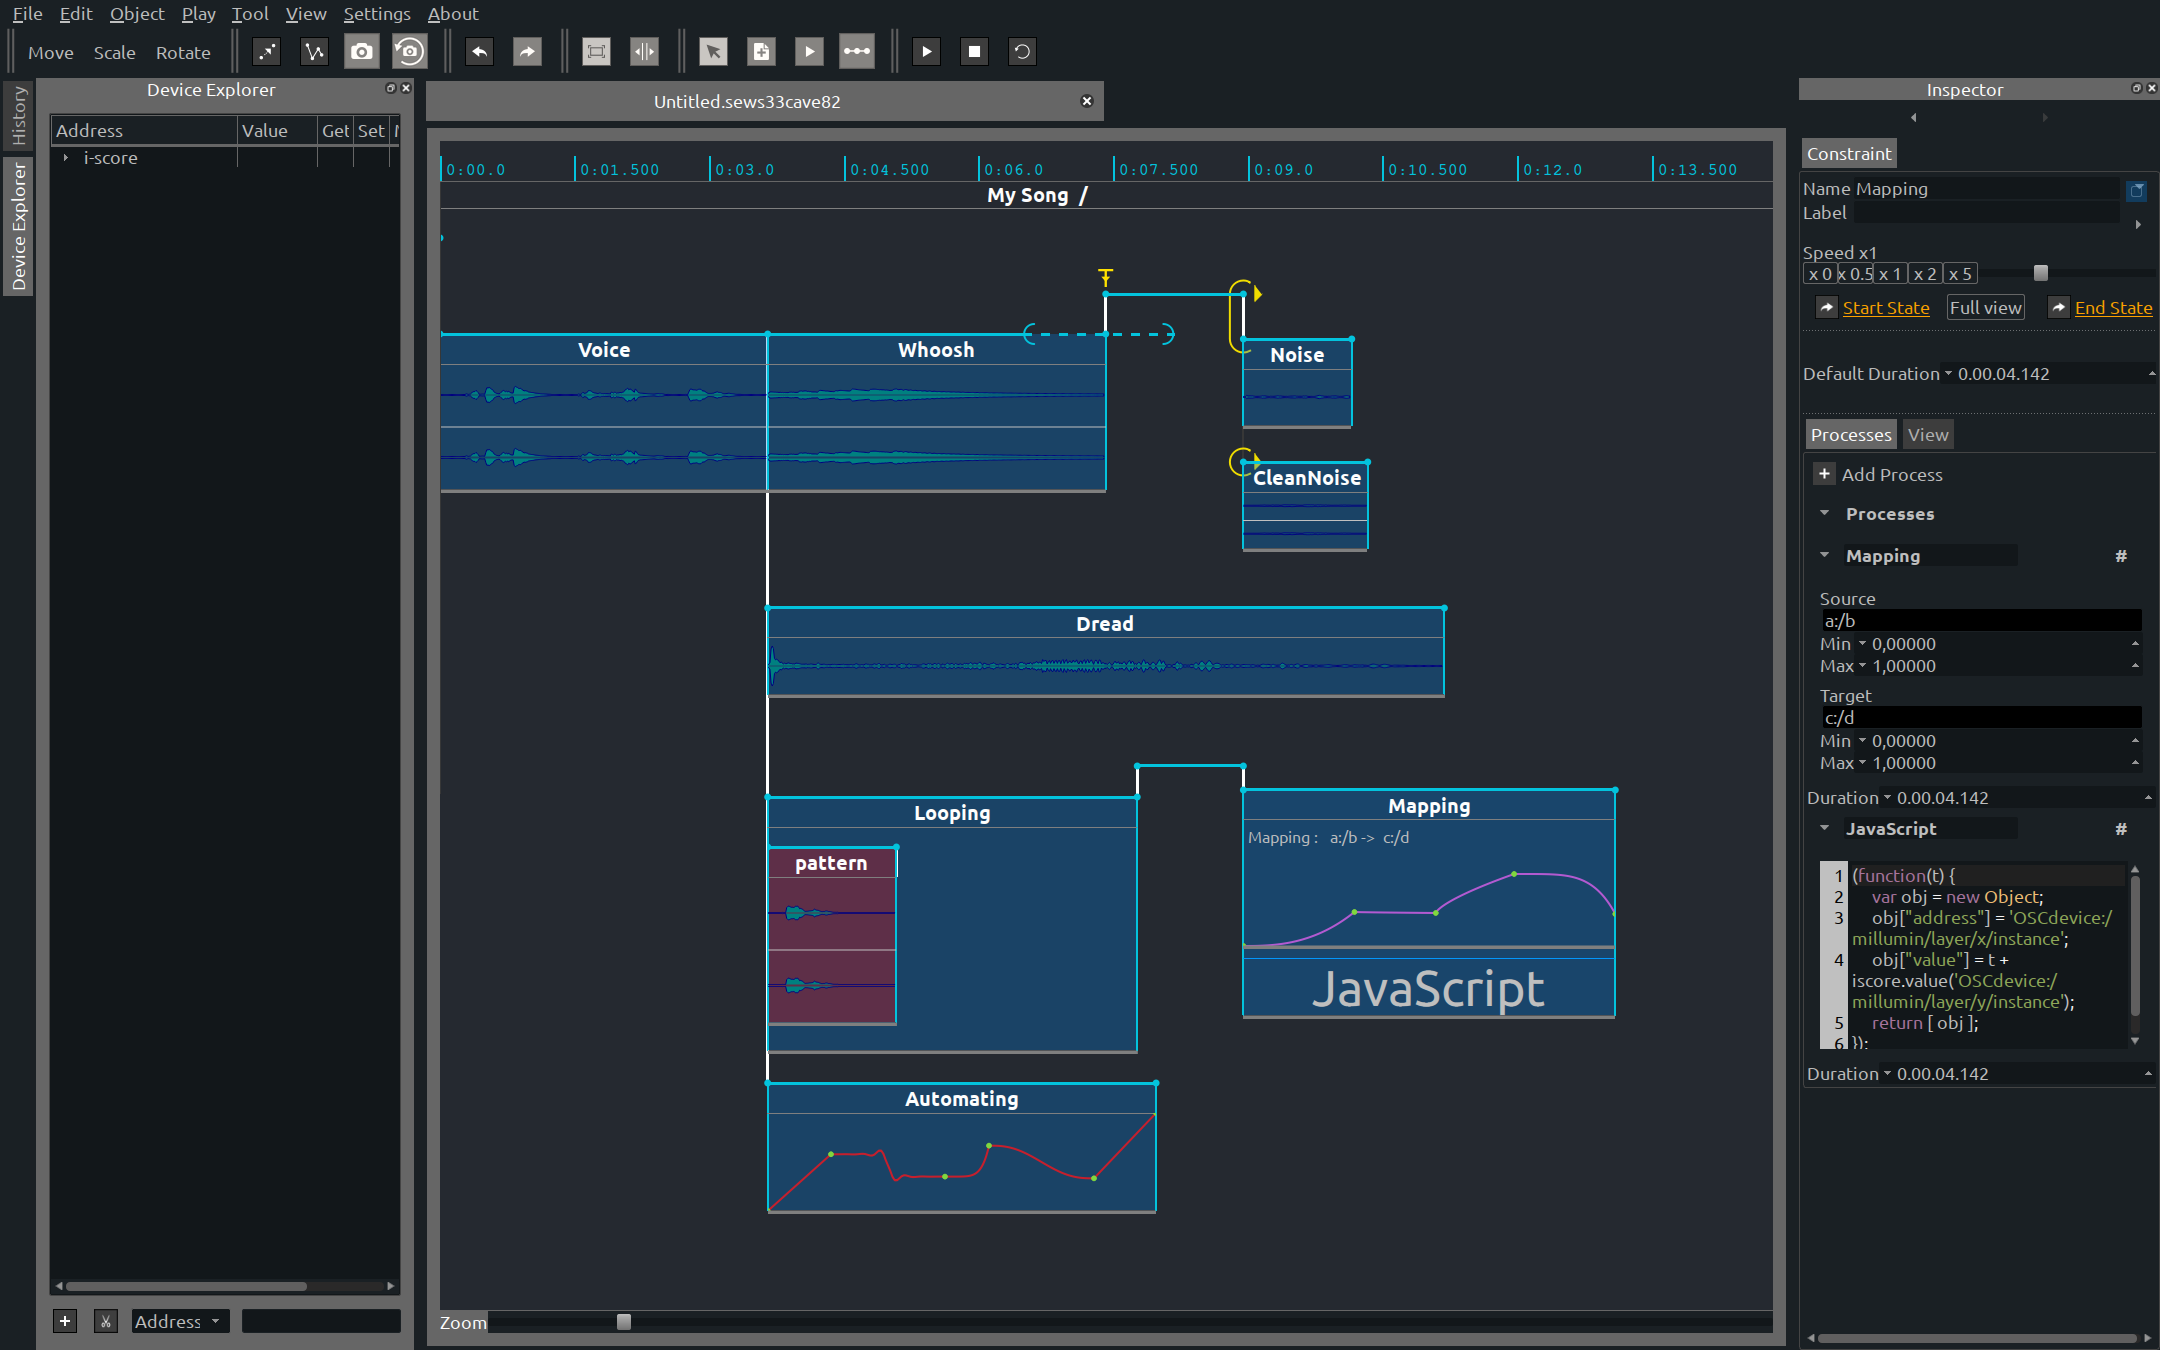
\includegraphics[width=\textwidth]{images/screens/12.png}
    \end{figure}
\end{frame}
\begin{frame} 
    \Large
    \begin{figure}
        \centering
        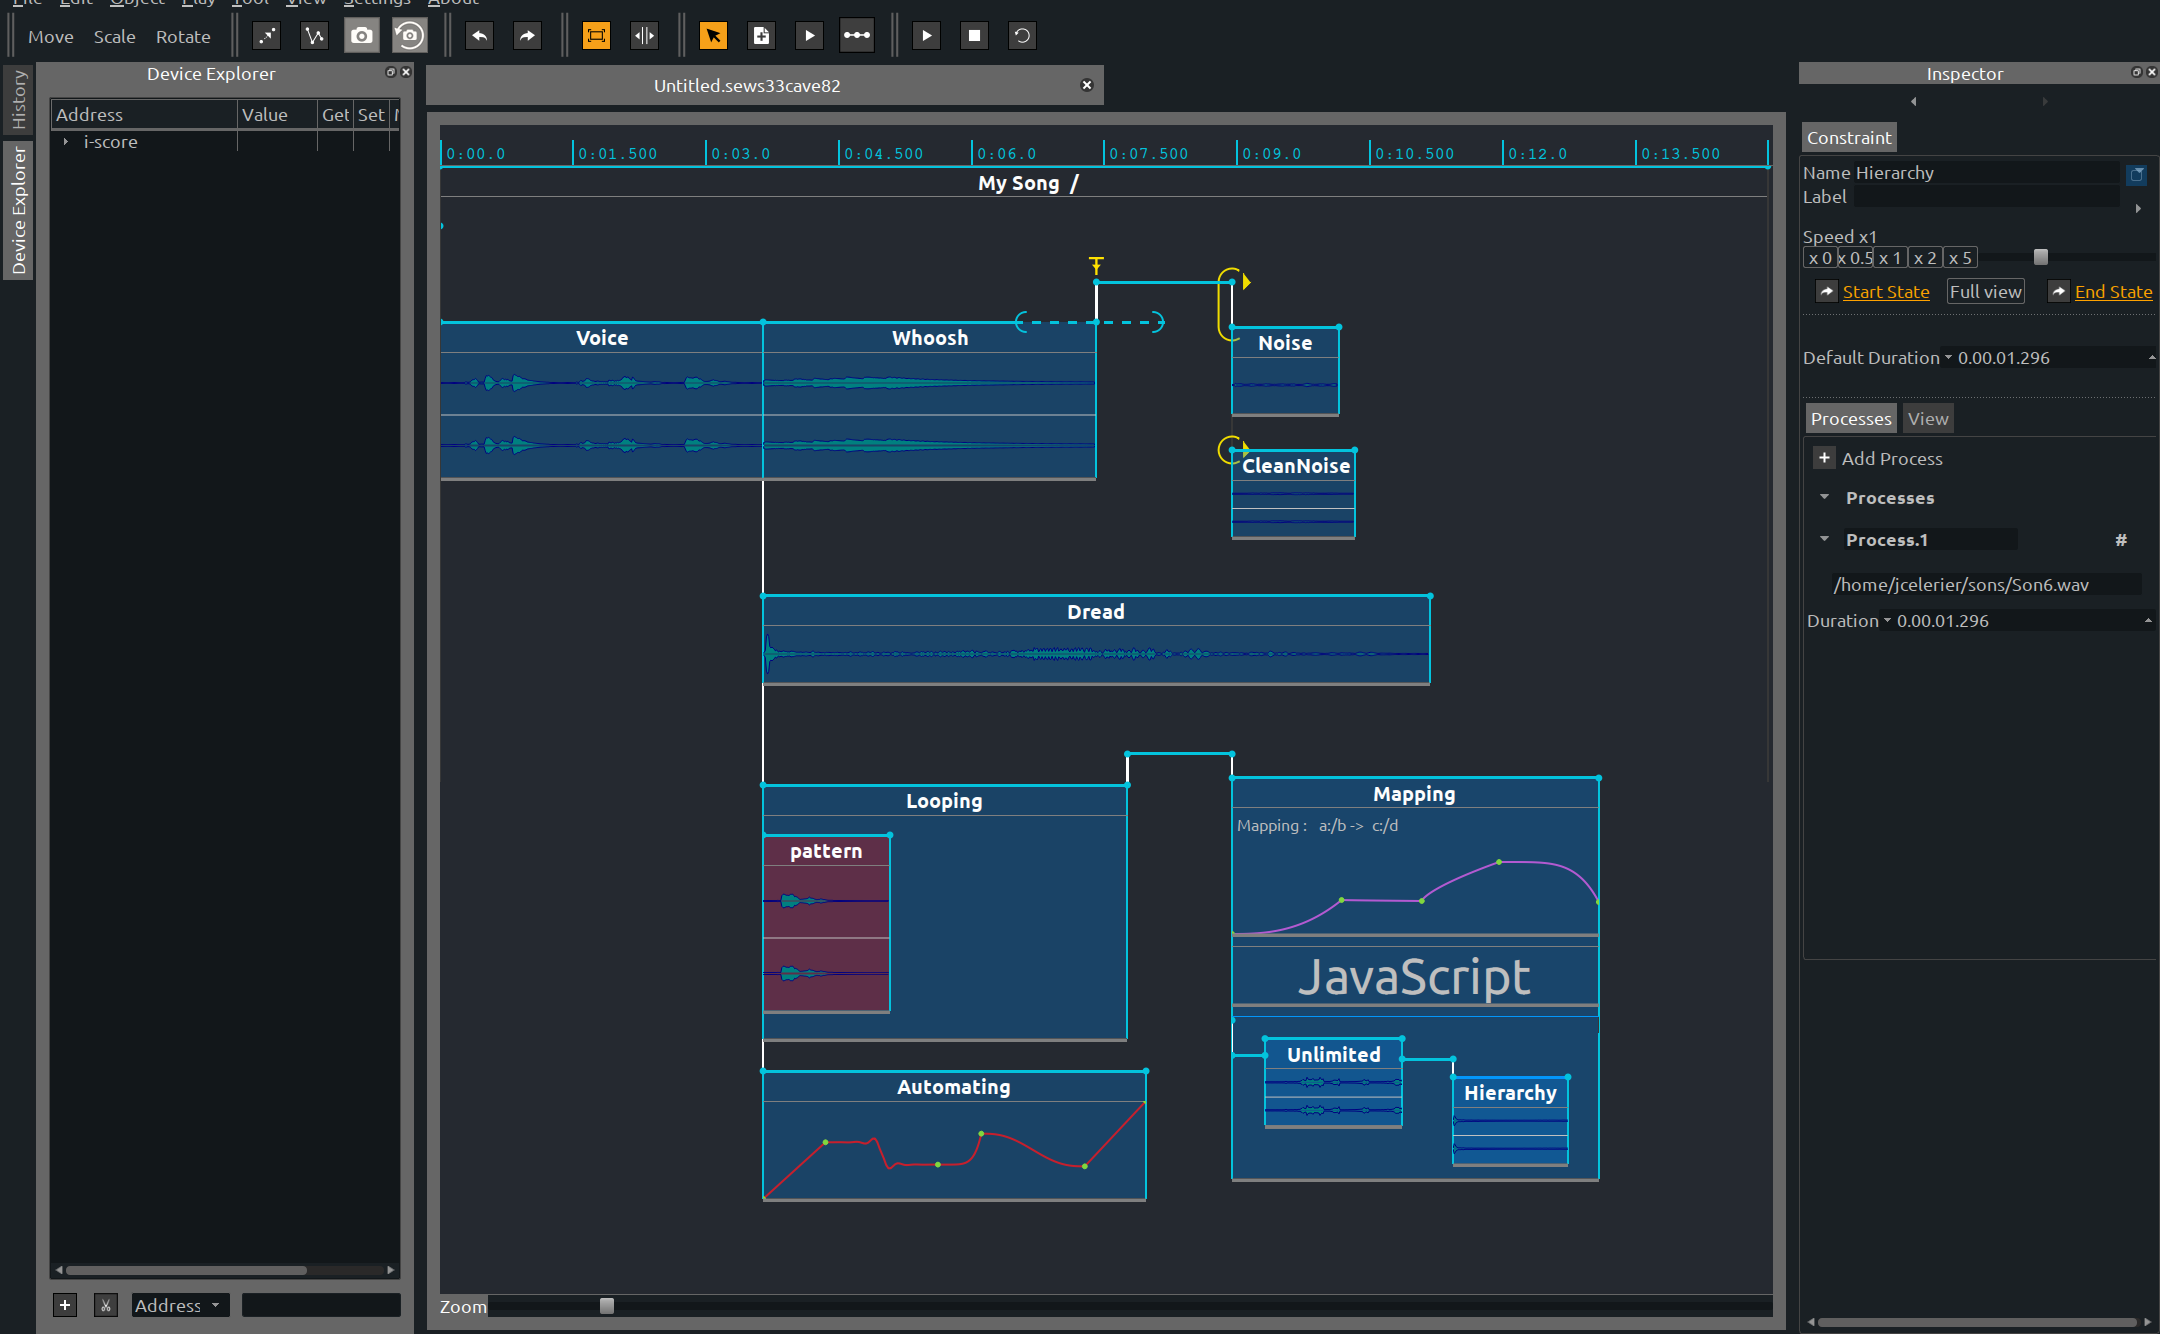
\includegraphics[width=\textwidth]{images/screens/13.png}
    \end{figure}
\end{frame}
\begin{frame} 
    \Large
    \begin{figure}
        \centering
        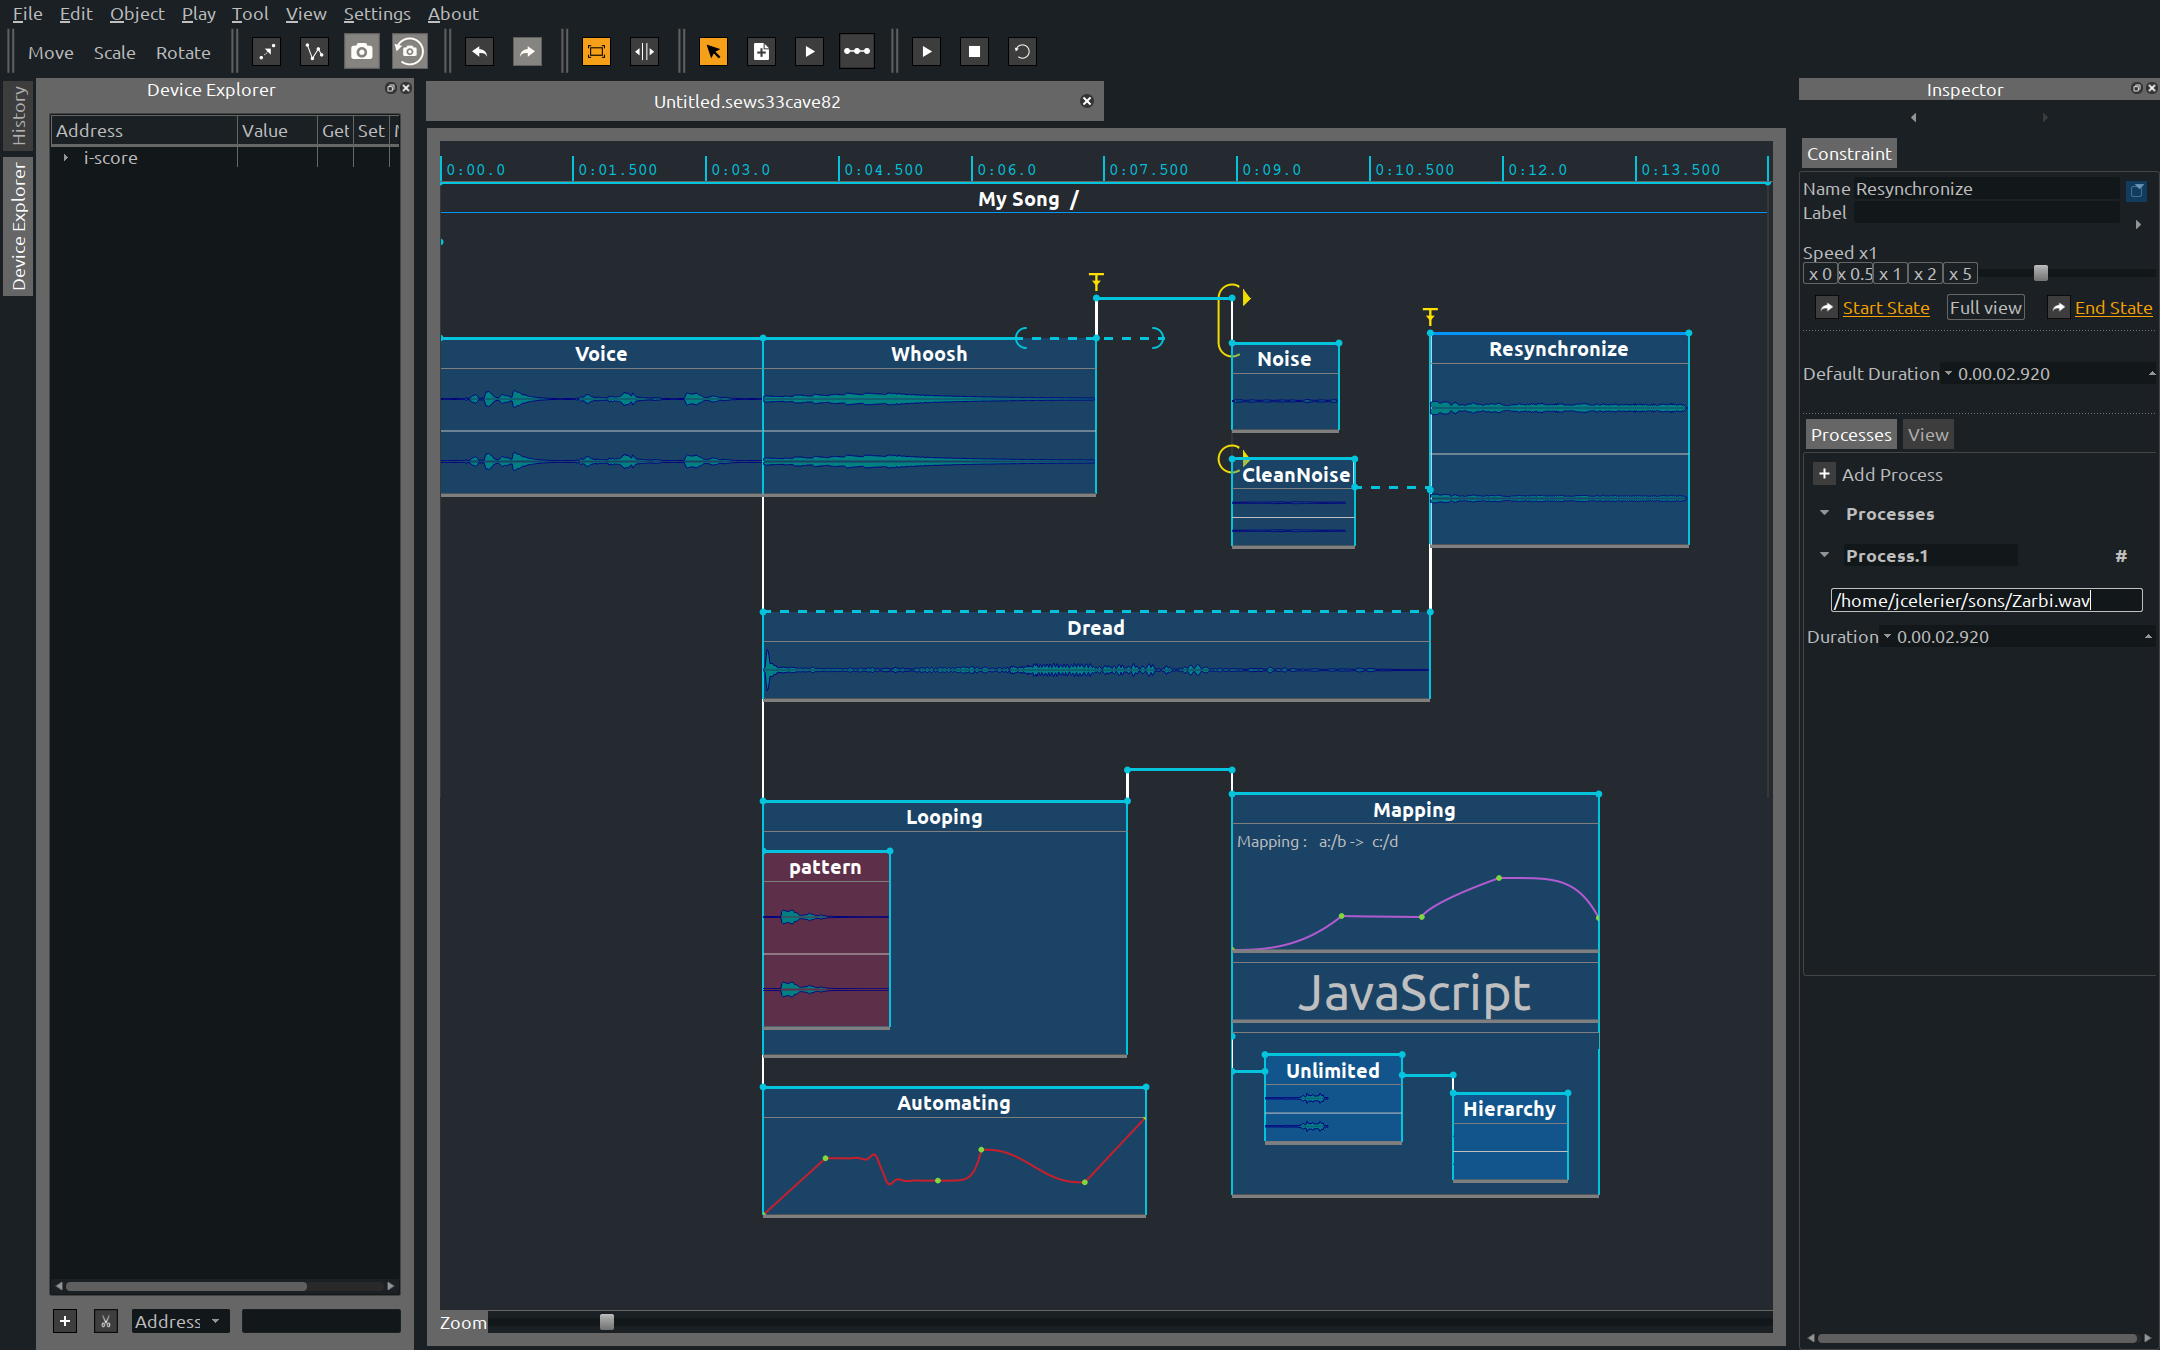
\includegraphics[width=\textwidth]{images/screens/14.png}
    \end{figure}
\end{frame}

\section{Description}

\begin{frame}	
    \frametitle{Origin}    
    \Large
    \begin{itemize}
        \item \textbf{i-score}~\\ \url{i-score.org}~\\$\rightarrow$ software for interactive show control.~\\~\\
        \item \textbf{LibAudioStream}\\ \url{github.com/sletz/libaudiostream}~\\$\rightarrow$ sequencer-as-a-library.~\\~\\
        \item \textbf{Audio plug-in} for i-score.
    \end{itemize}   
     
\end{frame}


\begin{frame}
    \frametitle{Vocabulary}   
    \begin{figure}
        \centering
        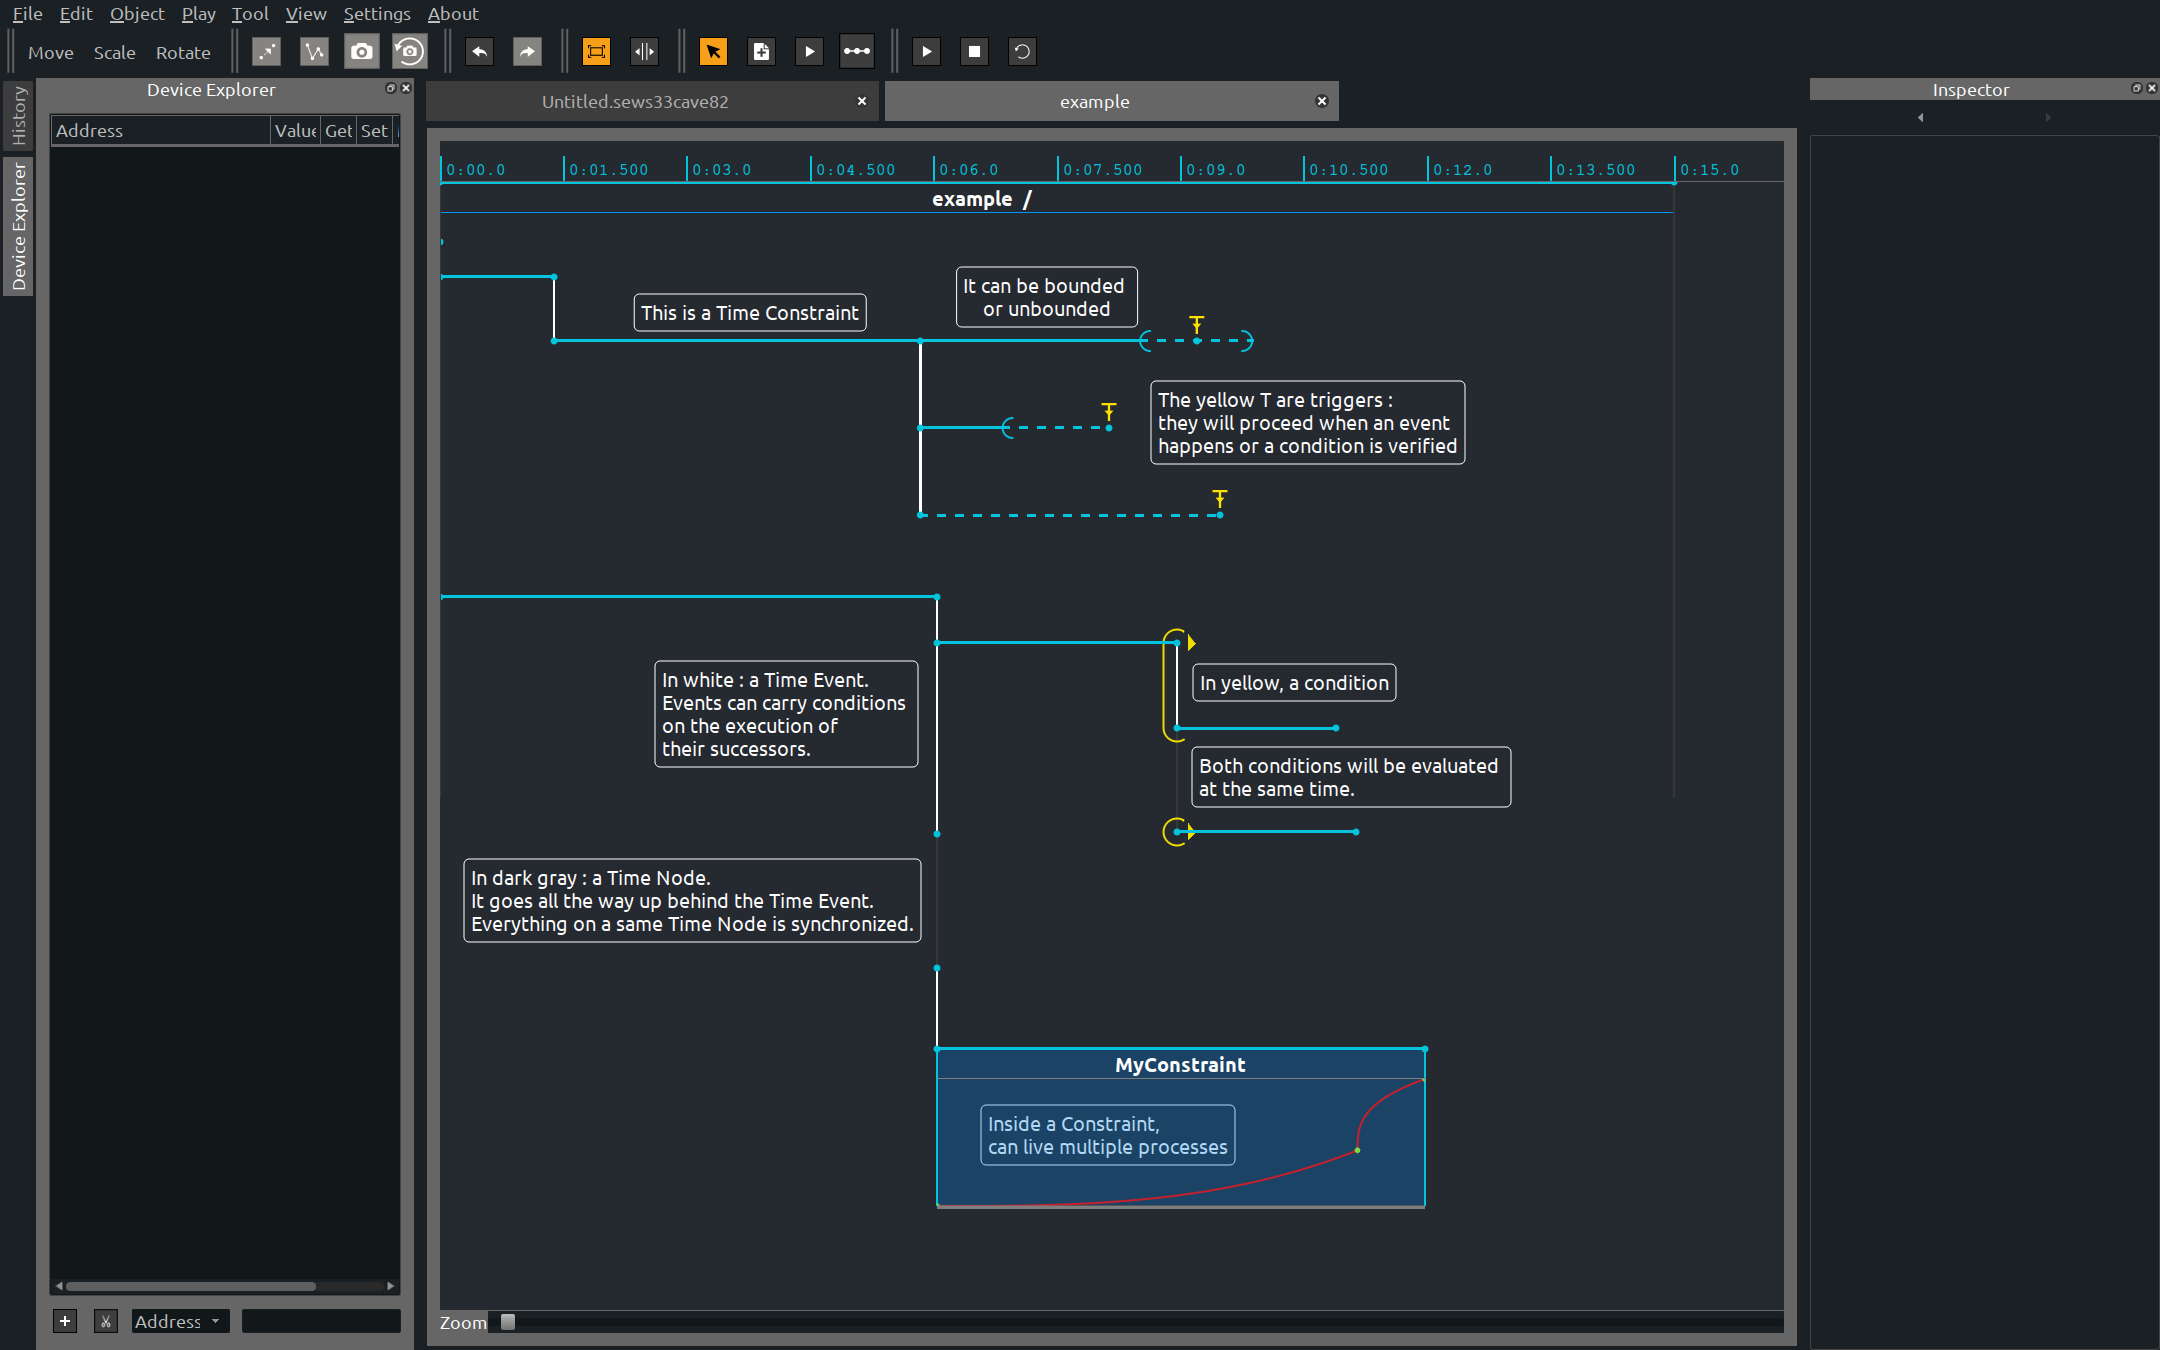
\includegraphics[width=\textwidth]{images/screens/example.png}
        \end{figure}
\end{frame}

\subsection{Audio processes}
\begin{frame}	
    \frametitle{Audio processes}    
    \Large
    \begin{itemize}
        \item Soundfile reading.
        \item Effect chains.
        \item Audiograph features : send and return audio from different points in the score.
        \item Mixing.
    \end{itemize}    
\end{frame}

\section{Method}
\begin{frame}
    \frametitle{The i-score audio graph}    
    \Large
    \begin{itemize}
        \item Audiostreams should be available for reading everywhere in the score : \\ $\rightarrow$ \textbf{flowgraph}.
        \item Not shown: it is not the main use case but a tool. UI focus is on the \textbf{temporal} aspect.
        \item For now the graph creation is \textbf{static}.
    \end{itemize}    
\end{frame}
\section{Demo}

\begin{frame}
    \frametitle{The i-score audio graph : mixing}    
	\Large
	
    Mixing unit : the temporal constraint.
    
    \begin{itemize}
        \item Each constraint mixes itself in its parent process.
        \item Each process mixes itself in its parent constraint.
    \end{itemize}
    
	\begin{figure}
		\centering
		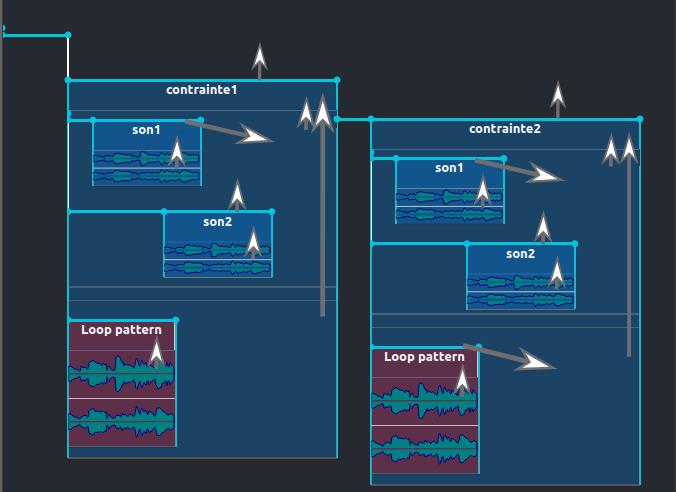
\includegraphics[width=0.6\textwidth]{images/mixage.png}
		\caption{Objects mix themselves together following the arrows}
	\end{figure}
\end{frame}

\begin{frame}
	\frametitle{Graphe de mixage}    
	\Large
	\begin{columns}
		\begin{column}{0.5\textwidth}
			\begin{figure}
				\centering
				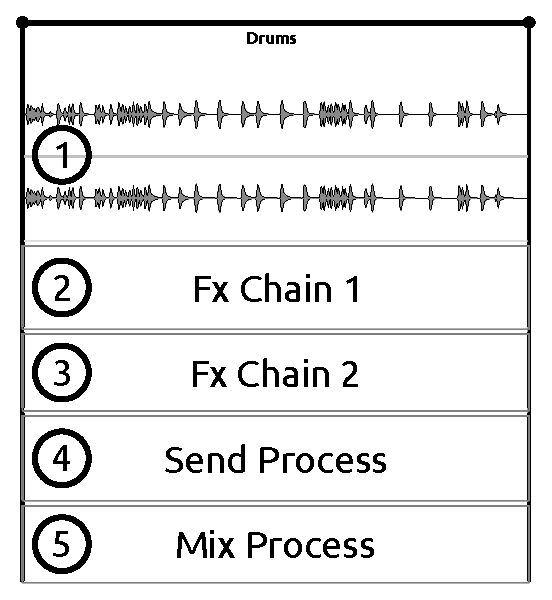
\includegraphics[width=\textwidth]{images/iscore1.eps}
				\caption{Une contrainte munie de 5 processus dans i-score}
			\end{figure}
		\end{column}
		\begin{column}{0.5\textwidth}
			\begin{figure}
				\centering
				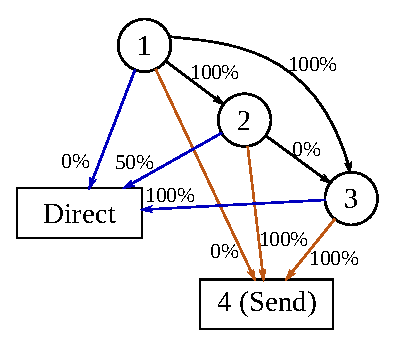
\includegraphics[width=\textwidth]{images/graph1.eps}
				\caption{La manière dont ces processus peuvent être traduits en graphe. 
					Le dosage est donné dans le \textbf{Mix Process}.}
			\end{figure}
		\end{column}
	\end{columns}
\end{frame}

\subsection{Graphes d'effets temporels}
\begin{frame}
	\frametitle{Audiographes}    
	\Large
	\begin{figure}
		\centering
		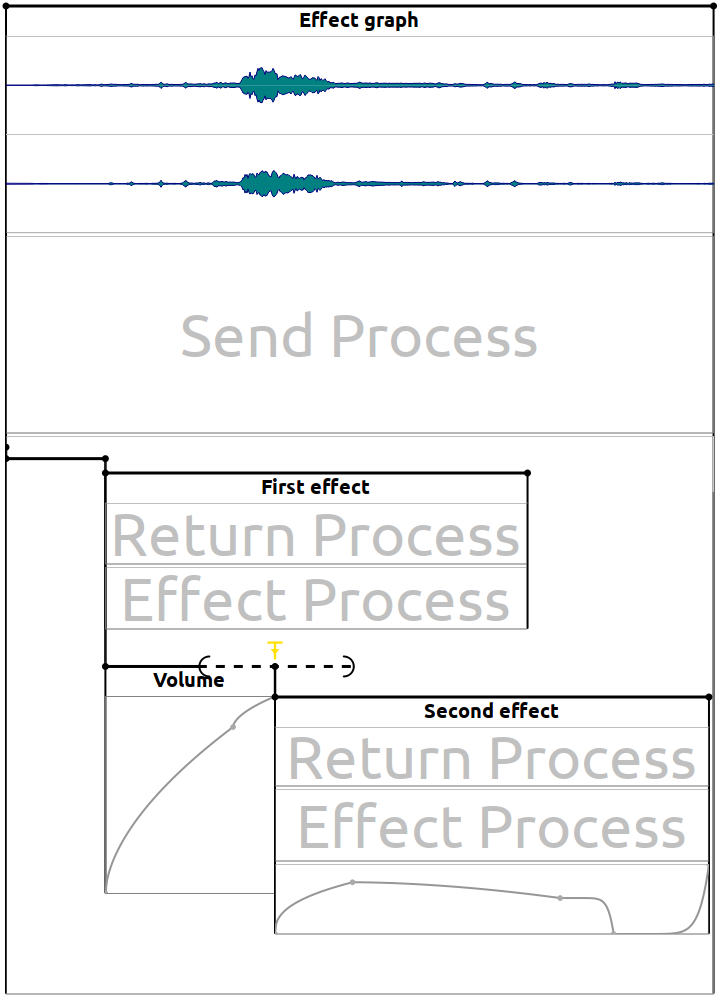
\includegraphics[width=0.4\textwidth]{images/ex3.png}
		\caption{Processus Send et Return pour partager un son entre plusieurs contraintes.}
	\end{figure}
\end{frame}

\section{Précision}
\begin{frame}
	\frametitle{Précision : cas des séquences}
	\Large
	
	\begin{columns}
		\begin{column}{0.5\textwidth}
			\begin{figure}
				\centering
				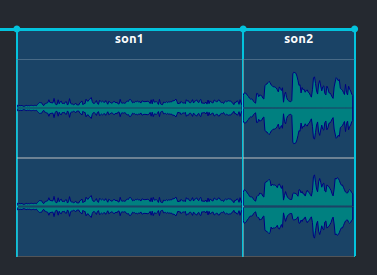
\includegraphics[width=\textwidth]{images/sequence.png}
				\caption{Le second son démarrera un échantillon après le dernier échantillon du premier son.}
			\end{figure}
		\end{column}
		\begin{column}{0.5\textwidth}
			\begin{figure}
				\centering
				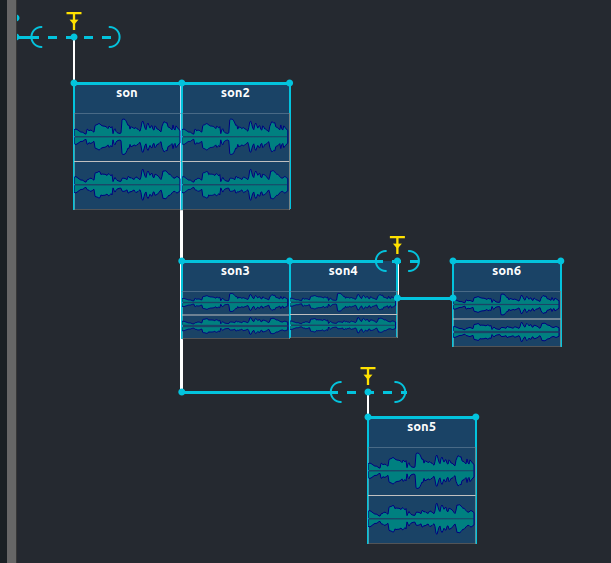
\includegraphics[width=\textwidth]{images/triggers.png}
				\caption{Lorsqu'un point d'interaction est déclenché, les nouvelles dates sont fixées jusqu'aux prochains points d'interaction}
			\end{figure}
		\end{column}
	\end{columns}
\end{frame}  

\begin{frame}
	\frametitle{Précision : cas des boucles}
	\Large
	
	\begin{columns}
		\begin{column}{0.5\textwidth}
			\begin{figure}
				\centering
				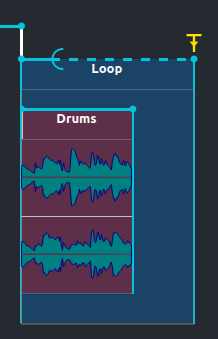
\includegraphics[width=0.62\textwidth]{images/loop.png}
				\caption{Chaque tour de boucle démarre un échantillon après le son précédent.}
			\end{figure}
		\end{column}
		\begin{column}{0.5\textwidth}
			\begin{figure}
				\centering
				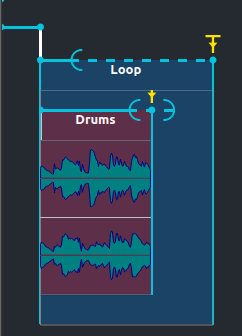
\includegraphics[width=0.7\textwidth]{images/loop2.png}
				\caption{Chaque tour de boucle démarre lors d'un déclenchement interactif.}
			\end{figure}
		\end{column}
	\end{columns}
\end{frame}  

\section{Introspection et effets}
\begin{frame}
	\frametitle{Introspection et effets}    
	\Large
	\begin{itemize}
		\item<1-> Actuellement : effets donnés en Faust.
		\item<2-> Chaque effet possède une liste de paramètres.
		\item<3-> Ces paramètres sont exposés dans l'arbre local d'i-score.
		\item<4-> Utilisables dans les automations, mappings, JS\dots
	\end{itemize}
	
	
	
\end{frame}

\begin{frame}
	\frametitle{Objectifs à venir} 
	\Large
	\begin{itemize}
		\item<1> Enregistrement, entrée audio.
		\item<2> Réutilisation en temps réel des enregistrements.
		\item<3> Meilleure intégration MIDI (piano roll ?).
		\item<4> Gestion des signatures temporelles.
		
	\end{itemize}
\end{frame}    

\begin{frame}
    \frametitle{Liens} 
    \Large
    \begin{itemize}
        \setlength\itemsep{1em}
        \item \textbf{Dépôt pour l'extension audio ({\unicodefun 🍎, 🐧})} :~\\
        \url{github.com/OSSIA/iscore-addon-audio}
        \item \textbf{Le logiciel} :~\\
         \url{i-score.org}
    \end{itemize}
        
    \centering
    \vspace{2em}
    \Large{Merci ! Questions ?}
    \vspace{2em}
    
    \tiny{Utilise le thème Beamer 'simple' de Facundo Muñoz; et les polices Fira, de Mozilla}
\end{frame}    

\begin{frame}
	\bibliographystyle{apalike}
	\bibliography{smc2016}
\end{frame}
\end{document}
